\documentclass[12pt,a4paper,twoside]{report}

% ============================================================================
% PACKAGES
% ============================================================================

% Language and fonts
\usepackage[utf8]{inputenc}
\usepackage[T1]{fontenc}
\usepackage[english]{babel}
\usepackage{textcomp}

% Page layout
\usepackage[
    a4paper,
    top=2.5cm,
    bottom=2.5cm,
    left=3cm,
    right=2.5cm,
    headheight=15pt
]{geometry}

% Graphics and colors
\usepackage{graphicx}
\usepackage{xcolor}
\usepackage{tikz}
\usepackage{pgfplots}
\pgfplotsset{compat=1.18}
\usetikzlibrary{
    shapes.geometric,
    shapes.symbols,
    shapes.arrows,
    shapes.multipart,
    arrows.meta,
    positioning,
    fit,
    backgrounds,
    shadows,
    calc,
    decorations.pathreplacing,
    decorations.pathmorphing,
    patterns,
    matrix,
    chains,
    trees
}

% Define custom colors
\definecolor{primary}{RGB}{0,102,204}
\definecolor{secondary}{RGB}{255,102,0}
\definecolor{accent}{RGB}{0,153,51}
\definecolor{warning}{RGB}{204,0,0}
\definecolor{rust}{RGB}{222,165,132}
\definecolor{success}{RGB}{40,167,69}
\definecolor{info}{RGB}{23,162,184}
\definecolor{lightgray}{RGB}{245,245,245}
\definecolor{mediumgray}{RGB}{200,200,200}
\definecolor{darkgray}{RGB}{100,100,100}

% Tables and lists
\usepackage{booktabs}
\usepackage{longtable}
\usepackage{array}
\usepackage{multirow}
\usepackage{enumitem}

% Code listings
\usepackage{listings}
\usepackage{tcolorbox}
\tcbuselibrary{skins,breakable,listings}

\lstdefinelanguage{Rust}{
    keywords={abstract, alignof, as, become, box, break, const, continue, crate, do, else, enum, extern, false, final, fn, for, if, impl, in, let, loop, macro, match, mod, move, mut, offsetof, override, priv, proc, pub, pure, ref, return, Self, self, sizeof, static, struct, super, trait, true, type, typeof, unsafe, unsized, use, virtual, where, while, yield, async, await, dyn},
    keywordstyle=\color{primary}\bfseries,
    ndkeywords={bool, u8, u16, u32, u64, u128, i8, i16, i32, i64, i128, f32, f64, usize, isize, char, str, String, Vec, Option, Result, Box, Rc, Arc, Cell, RefCell},
    ndkeywordstyle=\color{info}\bfseries,
    sensitive=true,
    comment=[l]{//},
    morecomment=[s]{/*}{*/},
    commentstyle=\color{success}\itshape,
    stringstyle=\color{secondary},
    morestring=[b]",
    morestring=[b]'
}

\lstdefinelanguage{toml}{
    keywords={true, false},
    keywordstyle=\color{primary}\bfseries,
    sensitive=true,
    comment=[l]{\#},
    commentstyle=\color{success}\itshape,
    stringstyle=\color{secondary},
    morestring=[b]",
    morestring=[b]'
}

\lstset{
    basicstyle=\ttfamily\small,
    breaklines=true,
    columns=flexible,
    numbers=left,
    numberstyle=\tiny\color{darkgray},
    frame=tb,
    framesep=5pt,
    backgroundcolor=\color{lightgray},
    rulecolor=\color{mediumgray},
    captionpos=b,
    commentstyle=\color{success}\itshape,
    keywordstyle=\color{primary}\bfseries,
    stringstyle=\color{secondary},
    showstringspaces=false
}

% Math
\usepackage{amsmath,amssymb,amsthm}

% References and links
\usepackage{hyperref}
\usepackage{cleveref}

\hypersetup{
    colorlinks=true,
    linkcolor=primary,
    filecolor=secondary,
    urlcolor=info,
    citecolor=accent,
    bookmarksnumbered=true,
    pdfauthor={GaussMeridian Development Team},
    pdftitle={GaussMeridian Code-Level Specifications v3.0},
    pdfsubject={Detailed Technical Specifications for GaussMeridian Implementation},
    pdfkeywords={GaussMeridian, Specifications, API, Rust, Implementation, Development}
}

% Headers and footers
\usepackage{fancyhdr}
\pagestyle{fancy}
\fancyhf{}
\fancyhead[LE]{\leftmark}
\fancyhead[RO]{\rightmark}
\fancyfoot[C]{\thepage}
\renewcommand{\headrulewidth}{0.4pt}
\renewcommand{\footrulewidth}{0.4pt}

% Custom commands
\newcommand{\gaussmeridian}{\textbf{GaussMeridian}}
\newcommand{\codeinline}[1]{\texttt{\small #1}}

% For checkmarks
\usepackage{pifont}
\newcommand{\cmark}{\ding{51}}
\newcommand{\xmark}{\ding{55}}

% Enhanced TikZ styles
\tikzset{
    component/.style={
        rectangle,
        draw=primary!80,
        fill=primary!15,
        rounded corners=4pt,
        minimum width=3.5cm,
        minimum height=1.2cm,
        text centered,
        font=\sffamily\small,
        drop shadow={shadow xshift=0.3ex, shadow yshift=-0.3ex, opacity=0.3},
        line width=0.8pt
    },
    module/.style={
        rectangle,
        draw=accent!70,
        fill=accent!12,
        rounded corners=3pt,
        minimum width=4cm,
        minimum height=1cm,
        font=\sffamily\small,
        text centered,
        line width=0.7pt
    },
    struct/.style={
        rectangle split,
        rectangle split parts=2,
        draw=info!70,
        fill=info!10,
        rounded corners=3pt,
        font=\ttfamily\footnotesize,
        line width=0.6pt
    },
    arrow/.style={
        ->,
        >=Stealth,
        thick,
        draw=darkgray,
        line width=0.9pt
    },
    dataflow/.style={
        ->,
        >=Stealth,
        thick,
        draw=accent!70,
        dashed,
        line width=0.9pt
    }
}

% ============================================================================
% DOCUMENT
% ============================================================================

\begin{document}

% ============================================================================
% TITLE PAGE
% ============================================================================

\begin{titlepage}
    \centering
    \vspace*{1.5cm}
    
    {\Huge\bfseries\color{primary} GaussMeridian\\[0.3cm]}
    {\huge\bfseries\color{primary} Code-Level Specifications\\[0.5cm]}
    {\LARGE\bfseries Technical Implementation Guide\\[2.5cm]}
    
    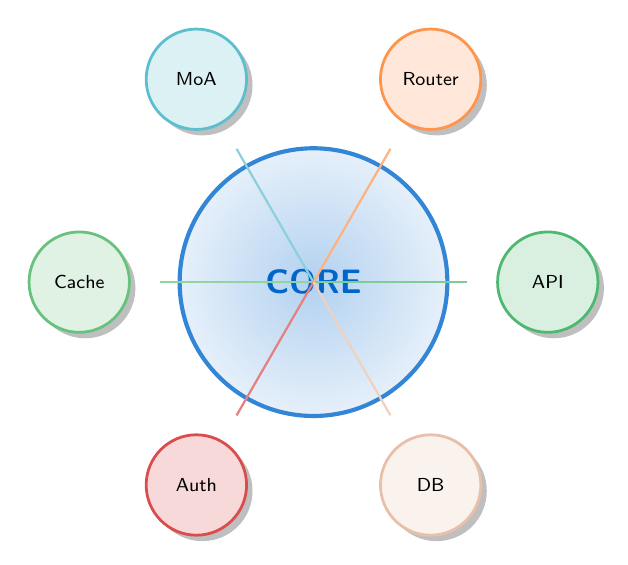
\begin{tikzpicture}[scale=0.85, transform shape]
        % Central module
        \shade[inner color=primary!30, outer color=primary!10] 
            (0,0) circle (2cm);
        \draw[primary!80, line width=1.5pt] (0,0) circle (2cm);
        \node[font=\Large\bfseries\sffamily, color=primary] at (0,0) {CORE};
        
        % Surrounding modules
        \foreach \angle/\text/\col in {
            0/API/accent,
            60/Router/secondary,
            120/MoA/info,
            180/Cache/success,
            240/Auth/warning,
            300/DB/rust%
        } {
            \node[circle, draw=\col!70, fill=\col!15, 
                  minimum size=1.5cm, drop shadow, line width=1pt,
                  font=\sffamily\footnotesize] 
                at (\angle:3.5cm) {\text};
            \draw[line width=0.8pt, draw=\col!50] 
                (0,0) -- (\angle:2.3cm);
        }
    \end{tikzpicture}
    
    \vspace{2cm}
    
    {\Large\bfseries Detailed Implementation Specifications\\[0.5cm]}
    {\large APIs $\bullet$ Data Structures $\bullet$ Interfaces $\bullet$ Protocols\\[0.8cm]}
    {\large Implementation Patterns $\bullet$ Best Practices\\[1.5cm]}
    
    {\large\bfseries Version 3.0 --- Production Ready\\[0.3cm]}
    {\large\today\\[2cm]}
    
    \vfill
    
    {\large\itshape\color{info}
    \textbf{For Development Teams}\\[0.2cm]
    Comprehensive Technical Reference
    }
\end{titlepage}

% ============================================================================
% EXECUTIVE SUMMARY
% ============================================================================

\chapter*{Executive Summary}
\addcontentsline{toc}{chapter}{Executive Summary}

\section*{Purpose and Scope}

This document provides comprehensive code-level specifications for the GaussMeridian Ecosystem, targeting software developers, technical architects, and DevOps engineers implementing or extending the platform. While the main architecture document focuses on system design and strategic decisions, this specification document details the concrete implementation requirements, API contracts, data structures, and coding patterns necessary for successful development.

\section*{Document Organization}

This specification is organized into logical development domains:

\textbf{Core Infrastructure} defines fundamental types, traits, error handling, and configuration systems that form the foundation of all other components.

\textbf{API Gateway Specifications} detail the HTTP API contracts, request/response formats, authentication flows, and middleware implementations.

\textbf{Routing Engine Specifications} describe routing strategy interfaces, model selection algorithms, circuit breaker implementations, and failover mechanisms.

\textbf{Multi-Agent Orchestration} specifies the GaussMoA subsystem including strategy interfaces, agent coordination protocols, and aggregation algorithms.

\textbf{Database Layer} defines the SurrealDB schema, query patterns, transaction management, and caching strategies.

\textbf{Security Implementation} specifies authentication mechanisms, authorization policies, encryption standards, and security best practices.

\textbf{Observability Infrastructure} details metrics collection, structured logging, distributed tracing, and monitoring integration.

\section*{Development Standards}

All code must adhere to the following standards:

\begin{itemize}[leftmargin=*]
    \item \textbf{Language Standards}: Rust 2021 edition, following official style guidelines
    \item \textbf{Type Safety}: Leverage Rust's type system to prevent errors at compile time
    \item \textbf{Error Handling}: Use Result types consistently, provide context in errors
    \item \textbf{Documentation}: All public APIs must have rustdoc comments with examples
    \item \textbf{Testing}: Minimum 80\% code coverage, unit tests for all public functions
    \item \textbf{Performance}: Profile critical paths, optimize allocations
    \item \textbf{Security}: Follow OWASP guidelines, validate all inputs
    \item \textbf{Async Patterns}: Use Tokio async runtime consistently
\end{itemize}

\section*{Key Technologies}

\begin{table}[h]
\centering
\begin{tabular}{@{}p{4cm}p{3cm}p{5cm}@{}}
\toprule
\textbf{Component} & \textbf{Technology} & \textbf{Version Requirement} \\
\midrule
Language & Rust & 1.75+ (2021 edition) \\
HTTP Framework & Axum & 0.7+ \\
Async Runtime & Tokio & 1.35+ \\
Serialization & Serde & 1.0+ \\
Database & SurrealDB & 2.0+ \\
Caching & Moka & 0.12+ \\
HTTP Client & Reqwest & 0.11+ \\
Metrics & Prometheus & 0.13+ \\
Logging & Tracing & 0.1+ \\
Testing & Tokio Test & 1.35+ \\
\bottomrule
\end{tabular}
\caption{Technology Stack Requirements}
\label{tab:tech-stack}
\end{table}

\tableofcontents
\listoffigures
\listoftables
\lstlistoflistings

% ============================================================================
% CHAPTER 1: CORE INFRASTRUCTURE
% ============================================================================

\chapter{Core Infrastructure Specifications}

\section{Project Structure}

The GaussMeridian codebase follows a modular workspace structure optimizing for maintainability and independent compilation.

\begin{lstlisting}[language=bash,caption={Project Directory Structure}]
gaussmeridian/
|-- Cargo.toml              # Workspace definition
|-- crates/
|   |-- gaussmeridian-core/   # Core types and traits
|   |-- gaussmeridian-api/    # HTTP API gateway
|   |-- gaussmeridian-router/ # Routing engine
|   |-- gaussmeridian-moa/    # Multi-agent orchestration
|   |-- gaussmeridian-db/     # Database layer
|   |-- gaussmeridian-cache/  # Caching subsystem
|   |-- gaussmeridian-auth/   # Authentication/authorization
|   |-- gaussmeridian-metrics/# Observability
|   `-- gaussmeridian-config/ # Configuration management
|-- services/
|   |-- server/             # Main API server
|   |-- webui/              # Deno/Fresh web console
|   `-- tui/                # Ratatui terminal interface
|-- tests/
|   |-- integration/        # Integration tests
|   `-- e2e/                # End-to-end tests
`-- docs/
    |-- api/                # API documentation
    `-- development/        # Developer guides
\end{lstlisting}

\subsection{Workspace Cargo.toml}

\begin{lstlisting}[language=toml,caption={Workspace Configuration}]
[workspace]
members = [
    "crates/gaussmeridian-core",
    "crates/gaussmeridian-api",
    "crates/gaussmeridian-router",
    "crates/gaussmeridian-moa",
    "crates/gaussmeridian-db",
    "crates/gaussmeridian-cache",
    "crates/gaussmeridian-auth",
    "crates/gaussmeridian-metrics",
    "crates/gaussmeridian-config",
    "services/server",
]

[workspace.package]
version = "3.0.0"
edition = "2021"
license = "AGPL-3.0-only"
repository = "https://github.com/gaussmeridian/gaussmeridian"

[workspace.dependencies]
# Async runtime
tokio = { version = "1.35", features = ["full"] }
tokio-util = "0.7"

# HTTP framework
axum = { version = "0.7", features = ["macros"] }
tower = "0.4"
tower-http = { version = "0.5", features = ["trace", "cors"] }

# Serialization
serde = { version = "1.0", features = ["derive"] }
serde_json = "1.0"

# Database
surrealdb = "2.0"

# Caching
moka = { version = "0.12", features = ["future"] }

# HTTP client
reqwest = { version = "0.11", features = ["json"] }

# Metrics and tracing
tracing = "0.1"
tracing-subscriber = { version = "0.3", features = ["env-filter"] }
metrics = "0.21"
metrics-exporter-prometheus = "0.13"

# Error handling
anyhow = "1.0"
thiserror = "1.0"

# Utilities
uuid = { version = "1.6", features = ["v4", "serde"] }
chrono = { version = "0.4", features = ["serde"] }
\end{lstlisting}

\section{Core Types and Traits}

\subsection{Fundamental Types}

\begin{lstlisting}[language=Rust,caption={Core Type Definitions - crates/gaussmeridian-core/src/types.rs}]
use serde::{Deserialize, Serialize};
use std::fmt;
use uuid::Uuid;

/// Unique identifier for models
#[derive(Debug, Clone, Copy, PartialEq, Eq, Hash, Serialize, Deserialize)]
pub struct ModelId(Uuid);

impl ModelId {
    pub fn new() -> Self {
        Self(Uuid::new_v4())
    }
    
    pub fn from_string(s: &str) -> Result<Self, uuid::Error> {
        Ok(Self(Uuid::parse_str(s)?))
    }
}

impl fmt::Display for ModelId {
    fn fmt(&self, f: &mut fmt::Formatter<'_>) -> fmt::Result {
        write!(f, "{}", self.0)
    }
}

/// Unique identifier for providers
#[derive(Debug, Clone, Copy, PartialEq, Eq, Hash, Serialize, Deserialize)]
pub struct ProviderId(Uuid);

impl ProviderId {
    pub fn new() -> Self {
        Self(Uuid::new_v4())
    }
}

/// Unique identifier for tenants
#[derive(Debug, Clone, Copy, PartialEq, Eq, Hash, Serialize, Deserialize)]
pub struct TenantId(Uuid);

impl TenantId {
    pub fn new() -> Self {
        Self(Uuid::new_v4())
    }
}

/// Unique identifier for users
#[derive(Debug, Clone, Copy, PartialEq, Eq, Hash, Serialize, Deserialize)]
pub struct UserId(Uuid);

impl UserId {
    pub fn new() -> Self {
        Self(Uuid::new_v4())
    }
}

/// API request identifier for tracing
#[derive(Debug, Clone, Copy, PartialEq, Eq, Hash, Serialize, Deserialize)]
pub struct RequestId(Uuid);

impl RequestId {
    pub fn new() -> Self {
        Self(Uuid::new_v4())
    }
}

impl fmt::Display for RequestId {
    fn fmt(&self, f: &mut fmt::Formatter<'_>) -> fmt::Result {
        write!(f, "{}", self.0)
    }
}

/// Model capability flags
#[derive(Debug, Clone, Copy, PartialEq, Eq, Serialize, Deserialize)]
pub struct ModelCapabilities {
    pub supports_functions: bool,
    pub supports_vision: bool,
    pub supports_streaming: bool,
    pub max_tokens: u32,
    pub context_window: u32,
}

/// Model pricing information
#[derive(Debug, Clone, Copy, Serialize, Deserialize)]
pub struct ModelPricing {
    pub input_cost_per_1m: f64,
    pub output_cost_per_1m: f64,
    pub currency: Currency,
}

#[derive(Debug, Clone, Copy, Serialize, Deserialize)]
pub enum Currency {
    USD,
    EUR,
    GBP,
}

/// Model performance metrics
#[derive(Debug, Clone, Copy, Default, Serialize, Deserialize)]
pub struct ModelMetrics {
    pub avg_latency_ms: f64,
    pub p95_latency_ms: f64,
    pub p99_latency_ms: f64,
    pub success_rate: f64,
    pub total_requests: u64,
    pub total_tokens: u64,
}
\end{lstlisting}

\subsection{Result and Error Types}

\begin{lstlisting}[language=Rust,caption={Error Definitions - crates/gaussmeridian-core/src/error.rs}]
use thiserror::Error;
use std::fmt;

/// Main result type for GaussMeridian operations
pub type Result<T> = std::result::Result<T, GaussMeridianError>;

/// Comprehensive error type covering all failure modes
#[derive(Error, Debug)]
pub enum GaussMeridianError {
    /// Database operation failures
    #[error("Database error: {0}")]
    Database(#[from] DatabaseError),
    
    /// Authentication failures
    #[error("Authentication error: {0}")]
    Authentication(#[from] AuthError),
    
    /// Authorization failures
    #[error("Authorization error: {0}")]
    Authorization(String),
    
    /// Routing failures
    #[error("Routing error: {0}")]
    Routing(#[from] RoutingError),
    
    /// Provider communication failures
    #[error("Provider error: {0}")]
    Provider(#[from] ProviderError),
    
    /// Cache operation failures
    #[error("Cache error: {0}")]
    Cache(String),
    
    /// Configuration errors
    #[error("Configuration error: {0}")]
    Configuration(String),
    
    /// Validation errors
    #[error("Validation error: {0}")]
    Validation(String),
    
    /// Rate limiting errors
    #[error("Rate limit exceeded: {0}")]
    RateLimit(String),
    
    /// Internal errors
    #[error("Internal error: {0}")]
    Internal(String),
}

/// Database-specific errors
#[derive(Error, Debug)]
pub enum DatabaseError {
    #[error("Connection failed: {0}")]
    ConnectionFailed(String),
    
    #[error("Query failed: {0}")]
    QueryFailed(String),
    
    #[error("Transaction failed: {0}")]
    TransactionFailed(String),
    
    #[error("Record not found: {0}")]
    NotFound(String),
    
    #[error("Constraint violation: {0}")]
    ConstraintViolation(String),
}

/// Authentication-specific errors
#[derive(Error, Debug)]
pub enum AuthError {
    #[error("Invalid credentials")]
    InvalidCredentials,
    
    #[error("Token expired")]
    TokenExpired,
    
    #[error("Invalid token: {0}")]
    InvalidToken(String),
    
    #[error("Missing authentication")]
    MissingAuth,
    
    #[error("Insufficient permissions")]
    InsufficientPermissions,
}

/// Routing-specific errors
#[derive(Error, Debug)]
pub enum RoutingError {
    #[error("No available models")]
    NoAvailableModels,
    
    #[error("Model not found: {0}")]
    ModelNotFound(String),
    
    #[error("Provider unavailable: {0}")]
    ProviderUnavailable(String),
    
    #[error("Circuit breaker open: {0}")]
    CircuitBreakerOpen(String),
    
    #[error("Strategy execution failed: {0}")]
    StrategyFailed(String),
}

/// Provider communication errors
#[derive(Error, Debug)]
pub enum ProviderError {
    #[error("HTTP request failed: {0}")]
    RequestFailed(String),
    
    #[error("Invalid response: {0}")]
    InvalidResponse(String),
    
    #[error("API error: {status} - {message}")]
    ApiError { status: u16, message: String },
    
    #[error("Timeout after {0}ms")]
    Timeout(u64),
    
    #[error("Rate limited by provider")]
    RateLimited,
}

/// Convert errors to HTTP status codes
impl GaussMeridianError {
    pub fn status_code(&self) -> u16 {
        match self {
            Self::Authentication(_) => 401,
            Self::Authorization(_) => 403,
            Self::Validation(_) => 400,
            Self::RateLimit(_) => 429,
            Self::Database(DatabaseError::NotFound(_)) => 404,
            Self::Routing(RoutingError::ModelNotFound(_)) => 404,
            _ => 500,
        }
    }
    
    pub fn error_code(&self) -> &str {
        match self {
            Self::Authentication(_) => "AUTH_ERROR",
            Self::Authorization(_) => "AUTHZ_ERROR",
            Self::Validation(_) => "VALIDATION_ERROR",
            Self::RateLimit(_) => "RATE_LIMIT_EXCEEDED",
            Self::Database(_) => "DATABASE_ERROR",
            Self::Routing(_) => "ROUTING_ERROR",
            Self::Provider(_) => "PROVIDER_ERROR",
            Self::Cache(_) => "CACHE_ERROR",
            Self::Configuration(_) => "CONFIG_ERROR",
            Self::Internal(_) => "INTERNAL_ERROR",
        }
    }
}
\end{lstlisting}

\subsection{Core Traits}

\begin{lstlisting}[language=Rust,caption={Core Trait Definitions - crates/gaussmeridian-core/src/traits.rs}]
use async_trait::async_trait;
use crate::{Result, ModelId, ProviderId, RequestId};
use serde::{Deserialize, Serialize};

/// Trait for all routing strategies
#[async_trait]
pub trait RoutingStrategy: Send + Sync {
    /// Select the best model for a given request
    async fn select_model(
        &self,
        request: &RouteRequest,
        available_models: &[ModelInfo],
    ) -> Result<ModelId>;
    
    /// Get strategy name for metrics
    fn name(&self) -> &str;
    
    /// Get strategy configuration
    fn config(&self) -> &StrategyConfig;
}

/// Trait for provider clients
#[async_trait]
pub trait ProviderClient: Send + Sync {
    /// Send a completion request to the provider
    async fn complete(
        &self,
        request: CompletionRequest,
    ) -> Result<CompletionResponse>;
    
    /// Stream a completion response
    async fn complete_stream(
        &self,
        request: CompletionRequest,
    ) -> Result<CompletionStream>;
    
    /// Get provider identifier
    fn provider_id(&self) -> ProviderId;
    
    /// Health check
    async fn health_check(&self) -> Result<ProviderHealth>;
}

/// Trait for caching backends
#[async_trait]
pub trait CacheBackend: Send + Sync {
    /// Get a cached response
    async fn get(&self, key: &CacheKey) -> Result<Option<CachedResponse>>;
    
    /// Store a response in cache
    async fn set(
        &self,
        key: CacheKey,
        value: CachedResponse,
        ttl: std::time::Duration,
    ) -> Result<()>;
    
    /// Invalidate cache entries
    async fn invalidate(&self, pattern: &str) -> Result<()>;
    
    /// Get cache statistics
    async fn stats(&self) -> Result<CacheStats>;
}

/// Trait for multi-agent strategies
#[async_trait]
pub trait MoAStrategy: Send + Sync {
    /// Execute multi-agent orchestration
    async fn execute(
        &self,
        request: &MoARequest,
        agents: &[AgentClient],
    ) -> Result<MoAResponse>;
    
    /// Get strategy name
    fn name(&self) -> &str;
    
    /// Get expected quality improvement
    fn quality_improvement(&self) -> f64;
}

/// Common request structure for routing
#[derive(Debug, Clone, Serialize, Deserialize)]
pub struct RouteRequest {
    pub request_id: RequestId,
    pub messages: Vec<Message>,
    pub model: Option<String>,
    pub temperature: Option<f32>,
    pub max_tokens: Option<u32>,
    pub routing_strategy: Option<String>,
}

/// Model information for routing decisions
#[derive(Debug, Clone, Serialize, Deserialize)]
pub struct ModelInfo {
    pub id: ModelId,
    pub name: String,
    pub provider_id: ProviderId,
    pub capabilities: ModelCapabilities,
    pub pricing: ModelPricing,
    pub metrics: ModelMetrics,
    pub health: ModelHealth,
}

/// Model health status
#[derive(Debug, Clone, Copy, Serialize, Deserialize)]
pub enum ModelHealth {
    Healthy,
    Degraded,
    Unhealthy,
}

/// Strategy configuration
#[derive(Debug, Clone, Serialize, Deserialize)]
pub struct StrategyConfig {
    pub priority: u8,
    pub enabled: bool,
    pub parameters: serde_json::Value,
}

/// Completion request to providers
#[derive(Debug, Clone, Serialize, Deserialize)]
pub struct CompletionRequest {
    pub model: String,
    pub messages: Vec<Message>,
    pub temperature: Option<f32>,
    pub max_tokens: Option<u32>,
    pub stream: bool,
}

/// Message in conversation
#[derive(Debug, Clone, Serialize, Deserialize)]
pub struct Message {
    pub role: MessageRole,
    pub content: String,
}

#[derive(Debug, Clone, Copy, Serialize, Deserialize)]
#[serde(rename_all = "lowercase")]
pub enum MessageRole {
    System,
    User,
    Assistant,
}

/// Completion response from providers
#[derive(Debug, Clone, Serialize, Deserialize)]
pub struct CompletionResponse {
    pub id: String,
    pub model: String,
    pub choices: Vec<Choice>,
    pub usage: Usage,
}

#[derive(Debug, Clone, Serialize, Deserialize)]
pub struct Choice {
    pub index: u32,
    pub message: Message,
    pub finish_reason: Option<String>,
}

#[derive(Debug, Clone, Copy, Serialize, Deserialize)]
pub struct Usage {
    pub prompt_tokens: u32,
    pub completion_tokens: u32,
    pub total_tokens: u32,
}

/// Streaming response type
pub type CompletionStream = 
    std::pin::Pin<Box<dyn futures::Stream<Item = Result<StreamChunk>> + Send>>;

#[derive(Debug, Clone, Serialize, Deserialize)]
pub struct StreamChunk {
    pub delta: String,
    pub finish_reason: Option<String>,
}

/// Cache key for lookups
#[derive(Debug, Clone, Hash, Eq, PartialEq)]
pub struct CacheKey {
    pub model: String,
    pub messages_hash: String,
    pub parameters_hash: String,
}

/// Cached response
#[derive(Debug, Clone, Serialize, Deserialize)]
pub struct CachedResponse {
    pub response: CompletionResponse,
    pub cached_at: chrono::DateTime<chrono::Utc>,
}

/// Cache statistics
#[derive(Debug, Clone, Default, Serialize, Deserialize)]
pub struct CacheStats {
    pub hits: u64,
    pub misses: u64,
    pub size: u64,
    pub hit_rate: f64,
}

/// Provider health information
#[derive(Debug, Clone, Serialize, Deserialize)]
pub struct ProviderHealth {
    pub status: HealthStatus,
    pub latency_ms: f64,
    pub error_rate: f64,
    pub last_check: chrono::DateTime<chrono::Utc>,
}

#[derive(Debug, Clone, Copy, Serialize, Deserialize)]
pub enum HealthStatus {
    Healthy,
    Degraded,
    Unhealthy,
}

/// Multi-agent request
#[derive(Debug, Clone, Serialize, Deserialize)]
pub struct MoARequest {
    pub request_id: RequestId,
    pub messages: Vec<Message>,
    pub strategy: String,
    pub agents: Vec<String>,
}

/// Multi-agent response
#[derive(Debug, Clone, Serialize, Deserialize)]
pub struct MoAResponse {
    pub response: CompletionResponse,
    pub agent_responses: Vec<AgentResponse>,
    pub strategy_used: String,
    pub quality_score: f64,
}

#[derive(Debug, Clone, Serialize, Deserialize)]
pub struct AgentResponse {
    pub agent: String,
    pub response: CompletionResponse,
    pub confidence: f64,
}

/// Agent client for MoA
pub struct AgentClient {
    pub model_id: ModelId,
    pub provider_client: Box<dyn ProviderClient>,
}
\end{lstlisting}

\section{Configuration Management}

\subsection{Configuration Structure}

\begin{lstlisting}[language=Rust,caption={Configuration Types - crates/gaussmeridian-config/src/lib.rs}]
use serde::{Deserialize, Serialize};
use std::path::Path;
use std::time::Duration;

/// Main configuration structure
#[derive(Debug, Clone, Serialize, Deserialize)]
pub struct GaussMeridianConfig {
    pub server: ServerConfig,
    pub database: DatabaseConfig,
    pub cache: CacheConfig,
    pub routing: RoutingConfig,
    pub auth: AuthConfig,
    pub providers: ProvidersConfig,
    pub observability: ObservabilityConfig,
}

impl GaussMeridianConfig {
    /// Load configuration from file
    pub fn from_file<P: AsRef<Path>>(path: P) -> Result<Self, ConfigError> {
        let content = std::fs::read_to_string(path)?;
        let config: Self = toml::from_str(&content)?;
        config.validate()?;
        Ok(config)
    }
    
    /// Load from environment variables
    pub fn from_env() -> Result<Self, ConfigError> {
        envy::from_env().map_err(|e| ConfigError::EnvError(e.to_string()))
    }
    
    /// Validate configuration
    fn validate(&self) -> Result<(), ConfigError> {
        if self.server.port == 0 {
            return Err(ConfigError::InvalidConfig("Port cannot be 0".to_string()));
        }
        
        if self.database.url.is_empty() {
            return Err(ConfigError::InvalidConfig(
                "Database URL is required".to_string()
            ));
        }
        
        Ok(())
    }
}

/// Server configuration
#[derive(Debug, Clone, Serialize, Deserialize)]
pub struct ServerConfig {
    pub host: String,
    pub port: u16,
    pub max_connections: usize,
    pub request_timeout_ms: u64,
    pub shutdown_timeout_s: u64,
}

impl Default for ServerConfig {
    fn default() -> Self {
        Self {
            host: "0.0.0.0".to_string(),
            port: 3000,
            max_connections: 10000,
            request_timeout_ms: 30000,
            shutdown_timeout_s: 30,
        }
    }
}

/// Database configuration
#[derive(Debug, Clone, Serialize, Deserialize)]
pub struct DatabaseConfig {
    pub url: String,
    pub namespace: String,
    pub database: String,
    pub max_connections: u32,
    pub connection_timeout_ms: u64,
    pub query_timeout_ms: u64,
}

impl Default for DatabaseConfig {
    fn default() -> Self {
        Self {
            url: "ws://localhost:8000".to_string(),
            namespace: "gaussmeridian".to_string(),
            database: "production".to_string(),
            max_connections: 100,
            connection_timeout_ms: 5000,
            query_timeout_ms: 30000,
        }
    }
}

/// Cache configuration
#[derive(Debug, Clone, Serialize, Deserialize)]
pub struct CacheConfig {
    pub l1_capacity: usize,
    pub l2_ttl_s: u64,
    pub l3_similarity_threshold: f32,
    pub enabled: bool,
}

impl Default for CacheConfig {
    fn default() -> Self {
        Self {
            l1_capacity: 1000,
            l2_ttl_s: 3600,
            l3_similarity_threshold: 0.95,
            enabled: true,
        }
    }
}

/// Routing configuration
#[derive(Debug, Clone, Serialize, Deserialize)]
pub struct RoutingConfig {
    pub default_strategy: String,
    pub circuit_breaker: CircuitBreakerConfig,
    pub retry: RetryConfig,
}

impl Default for RoutingConfig {
    fn default() -> Self {
        Self {
            default_strategy: "cost_optimized".to_string(),
            circuit_breaker: CircuitBreakerConfig::default(),
            retry: RetryConfig::default(),
        }
    }
}

/// Circuit breaker configuration
#[derive(Debug, Clone, Serialize, Deserialize)]
pub struct CircuitBreakerConfig {
    pub failure_threshold: u32,
    pub timeout_s: u64,
    pub half_open_max_requests: u32,
}

impl Default for CircuitBreakerConfig {
    fn default() -> Self {
        Self {
            failure_threshold: 5,
            timeout_s: 30,
            half_open_max_requests: 3,
        }
    }
}

/// Retry configuration
#[derive(Debug, Clone, Serialize, Deserialize)]
pub struct RetryConfig {
    pub max_attempts: u32,
    pub initial_backoff_ms: u64,
    pub max_backoff_ms: u64,
    pub backoff_multiplier: f64,
}

impl Default for RetryConfig {
    fn default() -> Self {
        Self {
            max_attempts: 3,
            initial_backoff_ms: 100,
            max_backoff_ms: 5000,
            backoff_multiplier: 2.0,
        }
    }
}

/// Authentication configuration
#[derive(Debug, Clone, Serialize, Deserialize)]
pub struct AuthConfig {
    pub jwt_secret: String,
    pub jwt_expiration_s: u64,
    pub api_key_header: String,
    pub bcrypt_cost: u32,
}

impl Default for AuthConfig {
    fn default() -> Self {
        Self {
            jwt_secret: String::new(), // Must be set
            jwt_expiration_s: 3600,
            api_key_header: "X-API-Key".to_string(),
            bcrypt_cost: 12,
        }
    }
}

/// Provider configuration
#[derive(Debug, Clone, Serialize, Deserialize)]
pub struct ProvidersConfig {
    pub openai: Option<ProviderConfig>,
    pub anthropic: Option<ProviderConfig>,
    pub google: Option<ProviderConfig>,
    pub mistral: Option<ProviderConfig>,
}

#[derive(Debug, Clone, Serialize, Deserialize)]
pub struct ProviderConfig {
    pub api_key: String,
    pub base_url: Option<String>,
    pub timeout_ms: u64,
    pub max_retries: u32,
}

/// Observability configuration
#[derive(Debug, Clone, Serialize, Deserialize)]
pub struct ObservabilityConfig {
    pub metrics_port: u16,
    pub log_level: String,
    pub log_format: LogFormat,
    pub tracing_enabled: bool,
}

#[derive(Debug, Clone, Serialize, Deserialize)]
#[serde(rename_all = "lowercase")]
pub enum LogFormat {
    Json,
    Pretty,
    Compact,
}

impl Default for ObservabilityConfig {
    fn default() -> Self {
        Self {
            metrics_port: 9090,
            log_level: "info".to_string(),
            log_format: LogFormat::Json,
            tracing_enabled: true,
        }
    }
}

/// Configuration errors
#[derive(Debug, thiserror::Error)]
pub enum ConfigError {
    #[error("IO error: {0}")]
    Io(#[from] std::io::Error),
    
    #[error("Parse error: {0}")]
    Parse(#[from] toml::de::Error),
    
    #[error("Environment error: {0}")]
    EnvError(String),
    
    #[error("Invalid configuration: {0}")]
    InvalidConfig(String),
}
\end{lstlisting}

\subsection{Example Configuration File}

\begin{lstlisting}[caption={Example config.toml}]
[server]
host = "0.0.0.0"
port = 3000
max_connections = 10000
request_timeout_ms = 30000
shutdown_timeout_s = 30

[database]
url = "ws://localhost:8000"
namespace = "gaussmeridian"
database = "production"
max_connections = 100
connection_timeout_ms = 5000
query_timeout_ms = 30000

[cache]
l1_capacity = 1000
l2_ttl_s = 3600
l3_similarity_threshold = 0.95
enabled = true

[routing]
default_strategy = "cost_optimized"

[routing.circuit_breaker]
failure_threshold = 5
timeout_s = 30
half_open_max_requests = 3

[routing.retry]
max_attempts = 3
initial_backoff_ms = 100
max_backoff_ms = 5000
backoff_multiplier = 2.0

[auth]
jwt_secret = "your-secret-key-here"
jwt_expiration_s = 3600
api_key_header = "X-API-Key"
bcrypt_cost = 12

[providers.openai]
api_key = "sk-..."
timeout_ms = 30000
max_retries = 3

[providers.anthropic]
api_key = "sk-ant-..."
timeout_ms = 30000
max_retries = 3

[observability]
metrics_port = 9090
log_level = "info"
log_format = "json"
tracing_enabled = true
\end{lstlisting}

% ============================================================================
% CHAPTER 2: API GATEWAY SPECIFICATIONS
% ============================================================================

\chapter{API Gateway Specifications}

\section{HTTP API Structure}

\begin{figure}[h]
\centering
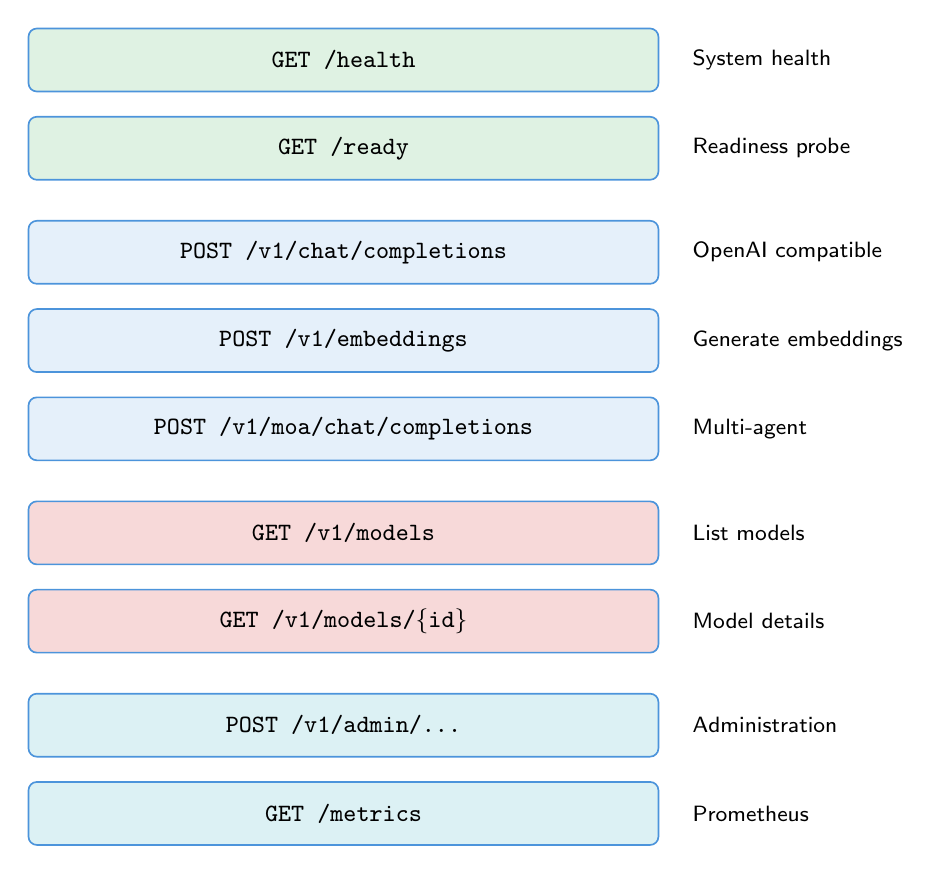
\begin{tikzpicture}[
    node distance=1.2cm,
    endpoint/.style={
        rectangle,
        draw=primary!70,
        fill=primary!10,
        rounded corners=3pt,
        minimum width=8cm,
        minimum height=0.8cm,
        font=\ttfamily\small,
        line width=0.6pt
    }
]
    \node[endpoint, fill=success!15] (health) {GET /health};
    \node[endpoint, below=0.3cm of health, fill=success!15] (ready) {GET /ready};
    \node[endpoint, below=0.5cm of ready] (complete) {POST /v1/chat/completions};
    \node[endpoint, below=0.3cm of complete] (embed) {POST /v1/embeddings};
    \node[endpoint, below=0.3cm of embed] (moa) {POST /v1/moa/chat/completions};
    \node[endpoint, below=0.5cm of moa, fill=warning!15] (models) {GET /v1/models};
    \node[endpoint, below=0.3cm of models, fill=warning!15] (model) {GET /v1/models/\{id\}};
    \node[endpoint, below=0.5cm of model, fill=info!15] (admin) {POST /v1/admin/...};
    \node[endpoint, below=0.3cm of admin, fill=info!15] (metrics) {GET /metrics};
    
    % Annotations
    \node[right=0.3cm of health, font=\sffamily\footnotesize] {System health};
    \node[right=0.3cm of ready, font=\sffamily\footnotesize] {Readiness probe};
    \node[right=0.3cm of complete, font=\sffamily\footnotesize] {OpenAI compatible};
    \node[right=0.3cm of embed, font=\sffamily\footnotesize] {Generate embeddings};
    \node[right=0.3cm of moa, font=\sffamily\footnotesize] {Multi-agent};
    \node[right=0.3cm of models, font=\sffamily\footnotesize] {List models};
    \node[right=0.3cm of model, font=\sffamily\footnotesize] {Model details};
    \node[right=0.3cm of admin, font=\sffamily\footnotesize] {Administration};
    \node[right=0.3cm of metrics, font=\sffamily\footnotesize] {Prometheus};
\end{tikzpicture}
\caption{API Endpoint Structure}
\label{fig:api-endpoints}
\end{figure}

\section{API Implementation}

\subsection{Main API Server}

\begin{lstlisting}[language=Rust,caption={API Server - crates/gaussmeridian-api/src/lib.rs}]
use axum::{
    extract::State,
    routing::{get, post},
    Router,
};
use std::sync::Arc;
use tower::ServiceBuilder;
use tower_http::{
    trace::TraceLayer,
    cors::CorsLayer,
    timeout::TimeoutLayer,
};
use gaussmeridian_core::Result;
use gaussmeridian_config::GaussMeridianConfig;

pub mod handlers;
pub mod middleware;
pub mod extractors;

/// Application state shared across handlers
#[derive(Clone)]
pub struct AppState {
    pub config: Arc<GaussMeridianConfig>,
    pub db: Arc<dyn DatabaseClient>,
    pub router: Arc<dyn RouterEngine>,
    pub moa: Arc<dyn MoAEngine>,
    pub cache: Arc<dyn CacheManager>,
    pub auth: Arc<dyn AuthService>,
}

/// Build the API router with all routes and middleware
pub fn build_router(state: AppState) -> Router {
    Router::new()
        // Health endpoints
        .route("/health", get(handlers::health::health_check))
        .route("/ready", get(handlers::health::ready_check))
        
        // Main API endpoints
        .route(
            "/v1/chat/completions",
            post(handlers::completions::create_completion)
        )
        .route(
            "/v1/embeddings",
            post(handlers::embeddings::create_embedding)
        )
        
        // Multi-agent endpoints
        .route(
            "/v1/moa/chat/completions",
            post(handlers::moa::moa_completion)
        )
        
        // Model endpoints
        .route("/v1/models", get(handlers::models::list_models))
        .route("/v1/models/:id", get(handlers::models::get_model))
        
        // Admin endpoints (protected)
        .route(
            "/v1/admin/models/:id",
            post(handlers::admin::update_model)
        )
        .route(
            "/v1/admin/users",
            get(handlers::admin::list_users)
        )
        
        // Metrics endpoint
        .route("/metrics", get(handlers::metrics::prometheus_metrics))
        
        // Middleware stack
        .layer(
            ServiceBuilder::new()
                .layer(TraceLayer::new_for_http())
                .layer(CorsLayer::permissive())
                .layer(TimeoutLayer::new(
                    std::time::Duration::from_millis(
                        state.config.server.request_timeout_ms
                    )
                ))
                .layer(axum::middleware::from_fn_with_state(
                    state.clone(),
                    middleware::auth::auth_middleware
                ))
                .layer(axum::middleware::from_fn(
                    middleware::request_id::request_id_middleware
                ))
        )
        .with_state(state)
}

/// Start the HTTP server
pub async fn serve(
    config: Arc<GaussMeridianConfig>,
    state: AppState,
) -> Result<()> {
    let app = build_router(state);
    
    let addr = format!("{}:{}", config.server.host, config.server.port);
    let listener = tokio::net::TcpListener::bind(&addr).await?;
    
    tracing::info!("Server listening on {}", addr);
    
    axum::serve(listener, app)
        .with_graceful_shutdown(shutdown_signal())
        .await?;
    
    Ok(())
}

/// Wait for shutdown signal
async fn shutdown_signal() {
    tokio::signal::ctrl_c()
        .await
        .expect("Failed to install CTRL+C signal handler");
    
    tracing::info!("Shutdown signal received");
}
\end{lstlisting}

\subsection{Completion Handler}

\begin{lstlisting}[language=Rust,caption={Chat Completions Handler - crates/gaussmeridian-api/src/handlers/completions.rs}]
use axum::{
    extract::State,
    http::StatusCode,
    Json,
};
use serde::{Deserialize, Serialize};
use gaussmeridian_core::{Result, RequestId, Message};
use crate::{AppState, extractors::RequestContext};

/// OpenAI-compatible completion request
#[derive(Debug, Deserialize)]
pub struct CompletionRequest {
    pub model: Option<String>,
    pub messages: Vec<Message>,
    pub temperature: Option<f32>,
    pub max_tokens: Option<u32>,
    pub top_p: Option<f32>,
    pub n: Option<u32>,
    pub stream: Option<bool>,
    pub stop: Option<Vec<String>>,
    pub presence_penalty: Option<f32>,
    pub frequency_penalty: Option<f32>,
    pub user: Option<String>,
    
    // GaussMeridian extensions
    pub routing_strategy: Option<String>,
    pub use_cache: Option<bool>,
}

/// OpenAI-compatible completion response
#[derive(Debug, Serialize)]
pub struct CompletionResponse {
    pub id: String,
    pub object: String,
    pub created: i64,
    pub model: String,
    pub choices: Vec<Choice>,
    pub usage: Usage,
    
    // GaussMeridian extensions
    #[serde(skip_serializing_if = "Option::is_none")]
    pub routing_info: Option<RoutingInfo>,
}

#[derive(Debug, Serialize)]
pub struct Choice {
    pub index: u32,
    pub message: Message,
    pub finish_reason: Option<String>,
}

#[derive(Debug, Serialize)]
pub struct Usage {
    pub prompt_tokens: u32,
    pub completion_tokens: u32,
    pub total_tokens: u32,
}

#[derive(Debug, Serialize)]
pub struct RoutingInfo {
    pub strategy_used: String,
    pub model_selected: String,
    pub provider: String,
    pub cache_hit: bool,
    pub latency_ms: u64,
}

/// Handle chat completion requests
#[tracing::instrument(skip(state, ctx))]
pub async fn create_completion(
    State(state): State<AppState>,
    ctx: RequestContext,
    Json(req): Json<CompletionRequest>,
) -> Result<Json<CompletionResponse>> {
    let start = std::time::Instant::now();
    
    // Validate request
    validate_request(&req)?;
    
    // Check cache if enabled
    if req.use_cache.unwrap_or(true) {
        if let Some(cached) = state.cache.get(&req).await? {
            tracing::info!("Cache hit for request");
            return Ok(Json(cached));
        }
    }
    
    // Route request
    let route_result = state.router.route(RouteRequest {
        request_id: ctx.request_id,
        messages: req.messages.clone(),
        model: req.model.clone(),
        temperature: req.temperature,
        max_tokens: req.max_tokens,
        routing_strategy: req.routing_strategy.clone(),
    }).await?;
    
    // Execute request with selected provider
    let response = route_result.provider_client
        .complete(CompletionRequest {
            model: route_result.model.name.clone(),
            messages: req.messages,
            temperature: req.temperature,
            max_tokens: req.max_tokens,
            stream: false,
        })
        .await?;
    
    let latency = start.elapsed();
    
    // Build response
    let result = CompletionResponse {
        id: response.id,
        object: "chat.completion".to_string(),
        created: chrono::Utc::now().timestamp(),
        model: route_result.model.name,
        choices: response.choices,
        usage: response.usage,
        routing_info: Some(RoutingInfo {
            strategy_used: route_result.strategy_used,
            model_selected: route_result.model.name.clone(),
            provider: route_result.provider.name.clone(),
            cache_hit: false,
            latency_ms: latency.as_millis() as u64,
        }),
    };
    
    // Update cache
    if req.use_cache.unwrap_or(true) {
        state.cache.set(&req, &result).await?;
    }
    
    // Record metrics
    metrics::counter!("completions_total", 1);
    metrics::histogram!("completion_latency_ms", latency.as_millis() as f64);
    
    Ok(Json(result))
}

/// Validate completion request
fn validate_request(req: &CompletionRequest) -> Result<()> {
    if req.messages.is_empty() {
        return Err(GaussMeridianError::Validation(
            "Messages array cannot be empty".to_string()
        ));
    }
    
    if let Some(temp) = req.temperature {
        if temp < 0.0 || temp > 2.0 {
            return Err(GaussMeridianError::Validation(
                "Temperature must be between 0 and 2".to_string()
            ));
        }
    }
    
    if let Some(max_tokens) = req.max_tokens {
        if max_tokens == 0 || max_tokens > 32000 {
            return Err(GaussMeridianError::Validation(
                "max_tokens must be between 1 and 32000".to_string()
            ));
        }
    }
    
    Ok(())
}
\end{lstlisting}

\subsection{Authentication Middleware}

\begin{lstlisting}[language=Rust,caption={Authentication Middleware - crates/gaussmeridian-api/src/middleware/auth.rs}]
use axum::{
    extract::{Request, State},
    http::{HeaderMap, StatusCode},
    middleware::Next,
    response::Response,
};
use gaussmeridian_auth::{AuthService, Claims};
use gaussmeridian_core::{Result, AuthError, UserId, TenantId};
use crate::AppState;

/// Authentication middleware
pub async fn auth_middleware(
    State(state): State<AppState>,
    headers: HeaderMap,
    mut request: Request,
    next: Next,
) -> Result<Response> {
    // Skip auth for health endpoints
    let path = request.uri().path();
    if path == "/health" || path == "/ready" {
        return Ok(next.run(request).await);
    }
    
    // Extract authentication credentials
    let auth_result = if let Some(api_key) = extract_api_key(&headers, &state) {
        state.auth.validate_api_key(&api_key).await
    } else if let Some(token) = extract_bearer_token(&headers) {
        state.auth.validate_jwt(&token).await
    } else {
        Err(AuthError::MissingAuth.into())
    };
    
    match auth_result {
        Ok(claims) => {
            // Add claims to request extensions
            request.extensions_mut().insert(claims);
            Ok(next.run(request).await)
        }
        Err(e) => {
            tracing::warn!("Authentication failed: {}", e);
            Err(e)
        }
    }
}

/// Extract API key from headers
fn extract_api_key(headers: &HeaderMap, state: &AppState) -> Option<String> {
    headers
        .get(&state.config.auth.api_key_header)
        .and_then(|v| v.to_str().ok())
        .map(|s| s.to_string())
}

/// Extract Bearer token from Authorization header
fn extract_bearer_token(headers: &HeaderMap) -> Option<String> {
    headers
        .get("authorization")
        .and_then(|v| v.to_str().ok())
        .and_then(|s| s.strip_prefix("Bearer "))
        .map(|s| s.to_string())
}

/// Request context extractor
#[derive(Debug, Clone)]
pub struct RequestContext {
    pub request_id: RequestId,
    pub user_id: UserId,
    pub tenant_id: TenantId,
    pub claims: Claims,
}

#[async_trait]
impl<S> FromRequestParts<S> for RequestContext
where
    S: Send + Sync,
{
    type Rejection = (StatusCode, String);
    
    async fn from_request_parts(
        parts: &mut Parts,
        _state: &S,
    ) -> Result<Self, Self::Rejection> {
        // Extract request ID
        let request_id = parts
            .extensions
            .get::<RequestId>()
            .ok_or_else(|| {
                (
                    StatusCode::INTERNAL_SERVER_ERROR,
                    "Missing request ID".to_string(),
                )
            })?
            .clone();
        
        // Extract claims
        let claims = parts
            .extensions
            .get::<Claims>()
            .ok_or_else(|| {
                (
                    StatusCode::UNAUTHORIZED,
                    "Missing authentication".to_string(),
                )
            })?
            .clone();
        
        Ok(Self {
            request_id,
            user_id: claims.user_id,
            tenant_id: claims.tenant_id,
            claims,
        })
    }
}
\end{lstlisting}

\section{Request/Response Flow}

\begin{figure}[p]
\centering
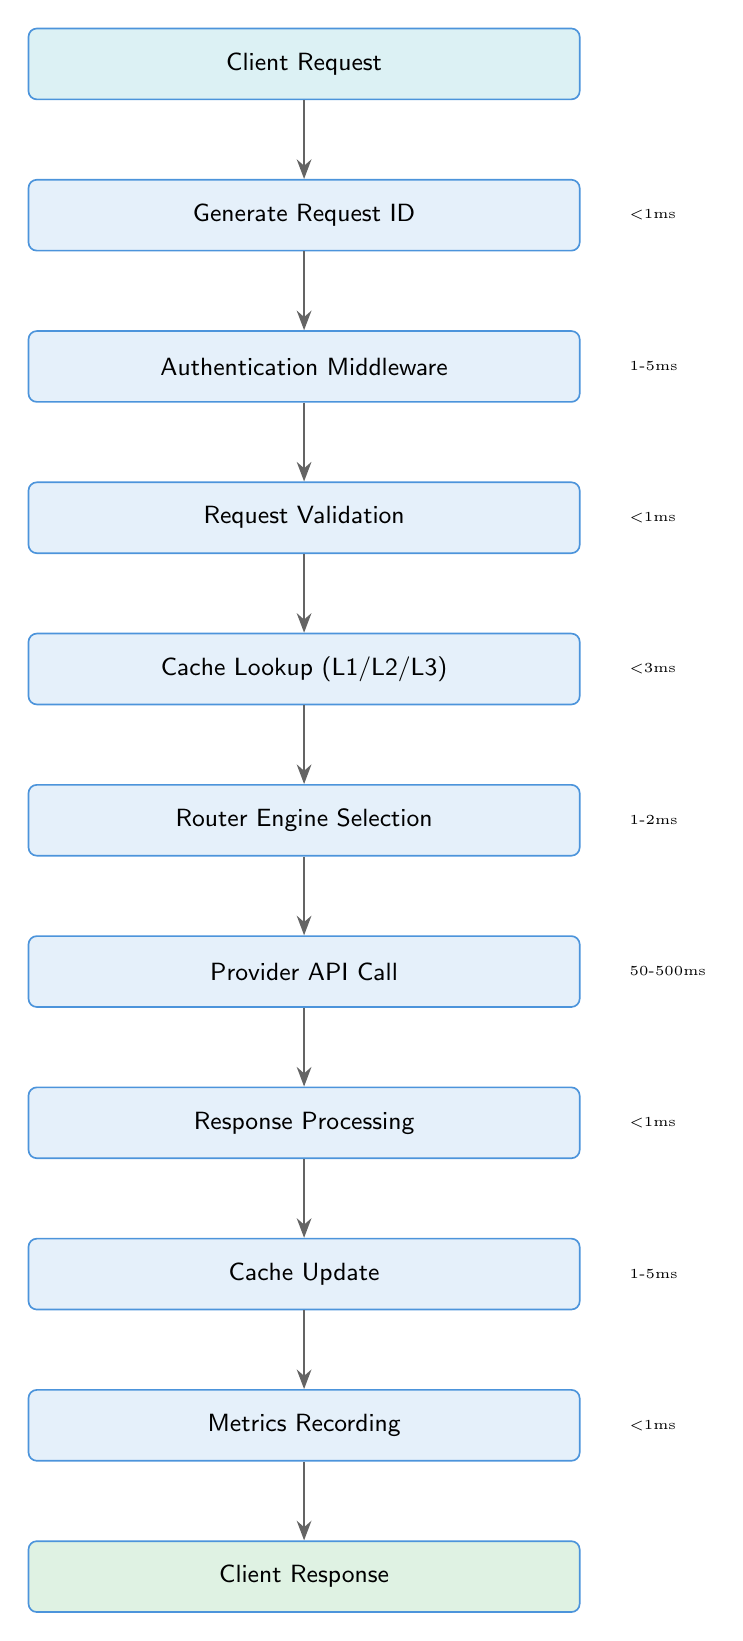
\begin{tikzpicture}[
    node distance=1cm,
    box/.style={
        rectangle,
        draw=primary!70,
        fill=primary!10,
        rounded corners=3pt,
        minimum width=7cm,
        minimum height=0.9cm,
        font=\sffamily\small,
        line width=0.6pt
    }
]
    \node[box, fill=info!15] (client) {Client Request};
    \node[box, below=of client] (reqid) {Generate Request ID};
    \node[box, below=of reqid] (auth) {Authentication Middleware};
    \node[box, below=of auth] (validate) {Request Validation};
    \node[box, below=of validate] (cache) {Cache Lookup (L1/L2/L3)};
    \node[box, below=of cache] (route) {Router Engine Selection};
    \node[box, below=of route] (provider) {Provider API Call};
    \node[box, below=of provider] (process) {Response Processing};
    \node[box, below=of process] (cacheset) {Cache Update};
    \node[box, below=of cacheset] (metrics) {Metrics Recording};
    \node[box, below=of metrics, fill=success!15] (response) {Client Response};
    
    % Arrows
    \foreach \from/\to in {
        client/reqid,
        reqid/auth,
        auth/validate,
        validate/cache,
        cache/route,
        route/provider,
        provider/process,
        process/cacheset,
        cacheset/metrics,
        metrics/response%
    } {
        \draw[arrow] (\from) -- (\to);
    }
    
    % Timing annotations
    \node[right=0.5cm of reqid, font=\tiny] {<1ms};
    \node[right=0.5cm of auth, font=\tiny] {1-5ms};
    \node[right=0.5cm of validate, font=\tiny] {<1ms};
    \node[right=0.5cm of cache, font=\tiny] {<3ms};
    \node[right=0.5cm of route, font=\tiny] {1-2ms};
    \node[right=0.5cm of provider, font=\tiny] {50-500ms};
    \node[right=0.5cm of process, font=\tiny] {<1ms};
    \node[right=0.5cm of cacheset, font=\tiny] {1-5ms};
    \node[right=0.5cm of metrics, font=\tiny] {<1ms};
\end{tikzpicture}
\caption{Complete Request/Response Flow with Timing}
\label{fig:request-flow}
\end{figure}

\subsection{Streaming Response Handler}

\begin{lstlisting}[language=Rust,caption={Streaming Completions - crates/gaussmeridian-api/src/handlers/streaming.rs}]
use axum::{
    extract::State,
    response::sse::{Event, Sse},
};
use futures::stream::{Stream, StreamExt};
use serde::{Deserialize, Serialize};
use gaussmeridian_core::{Result, CompletionStream};
use crate::AppState;

/// Server-Sent Events streaming response
pub async fn stream_completion(
    State(state): State<AppState>,
    ctx: RequestContext,
    Json(req): Json<CompletionRequest>,
) -> Result<Sse<impl Stream<Item = Result<Event>>>> {
    // Validate streaming is requested
    if !req.stream.unwrap_or(false) {
        return Err(GaussMeridianError::Validation(
            "Streaming not requested".to_string()
        ));
    }
    
    // Route request
    let route_result = state.router.route(RouteRequest {
        request_id: ctx.request_id,
        messages: req.messages.clone(),
        model: req.model.clone(),
        temperature: req.temperature,
        max_tokens: req.max_tokens,
        routing_strategy: req.routing_strategy.clone(),
    }).await?;
    
    // Get streaming response from provider
    let provider_stream = route_result.provider_client
        .complete_stream(CompletionRequest {
            model: route_result.model.name.clone(),
            messages: req.messages,
            temperature: req.temperature,
            max_tokens: req.max_tokens,
            stream: true,
        })
        .await?;
    
    // Transform provider stream to SSE events
    let event_stream = provider_stream
        .map(|chunk_result| {
            chunk_result.and_then(|chunk| {
                let event = StreamChunkEvent {
                    id: Uuid::new_v4().to_string(),
                    choices: vec![StreamChoice {
                        index: 0,
                        delta: StreamDelta {
                            content: Some(chunk.delta),
                            role: None,
                        },
                        finish_reason: chunk.finish_reason,
                    }],
                };
                
                let json = serde_json::to_string(&event)?;
                Ok(Event::default()
                    .data(json)
                    .event("message"))
            })
        });
    
    Ok(Sse::new(event_stream))
}

#[derive(Debug, Serialize)]
struct StreamChunkEvent {
    id: String,
    choices: Vec<StreamChoice>,
}

#[derive(Debug, Serialize)]
struct StreamChoice {
    index: u32,
    delta: StreamDelta,
    finish_reason: Option<String>,
}

#[derive(Debug, Serialize)]
struct StreamDelta {
    #[serde(skip_serializing_if = "Option::is_none")]
    content: Option<String>,
    #[serde(skip_serializing_if = "Option::is_none")]
    role: Option<String>,
}
\end{lstlisting}

\subsection{Error Response Handler}

\begin{lstlisting}[language=Rust,caption={Error Handling - crates/gaussmeridian-api/src/error.rs}]
use axum::{
    http::StatusCode,
    response::{IntoResponse, Response},
    Json,
};
use serde::Serialize;
use gaussmeridian_core::GaussMeridianError;

/// Error response format
#[derive(Debug, Serialize)]
pub struct ErrorResponse {
    pub error: ErrorDetail,
}

#[derive(Debug, Serialize)]
pub struct ErrorDetail {
    pub code: String,
    pub message: String,
    #[serde(skip_serializing_if = "Option::is_none")]
    pub details: Option<serde_json::Value>,
}

/// Implement IntoResponse for GaussMeridianError
impl IntoResponse for GaussMeridianError {
    fn into_response(self) -> Response {
        let status_code = StatusCode::from_u16(self.status_code())
            .unwrap_or(StatusCode::INTERNAL_SERVER_ERROR);
        
        let error_response = ErrorResponse {
            error: ErrorDetail {
                code: self.error_code().to_string(),
                message: self.to_string(),
                details: None,
            },
        };
        
        // Log error
        tracing::error!(
            error_code = self.error_code(),
            error = %self,
            "Request failed"
        );
        
        // Record metrics
        metrics::counter!(
            "errors_total",
            "error_type" => self.error_code()
        )
        .increment(1);
        
        (status_code, Json(error_response)).into_response()
    }
}
\end{lstlisting}

% ============================================================================
% CHAPTER 3: ROUTING ENGINE SPECIFICATIONS
% ============================================================================

\chapter{Routing Engine Specifications}

\section{Router Core Implementation}

\begin{lstlisting}[language=Rust,caption={Router Engine - crates/gaussmeridian-router/src/lib.rs}]
use async_trait::async_trait;
use gaussmeridian_core::{
    Result, RouteRequest, ModelInfo, ModelId, RoutingStrategy,
    ProviderClient, GaussMeridianError,
};
use std::sync::Arc;
use tokio::sync::RwLock;

/// Main router engine coordinating model selection
pub struct RouterEngine {
    strategies: RwLock<Vec<Arc<dyn RoutingStrategy>>>,
    providers: RwLock<Vec<Arc<dyn ProviderClient>>>,
    models: RwLock<Vec<ModelInfo>>,
    circuit_breakers: Arc<CircuitBreakerManager>,
}

impl RouterEngine {
    pub fn new(
        circuit_breakers: Arc<CircuitBreakerManager>,
    ) -> Self {
        Self {
            strategies: RwLock::new(Vec::new()),
            providers: RwLock::new(Vec::new()),
            models: RwLock::new(Vec::new()),
            circuit_breakers,
        }
    }
    
    /// Register a routing strategy
    pub async fn register_strategy(
        &self,
        strategy: Arc<dyn RoutingStrategy>,
    ) {
        self.strategies.write().await.push(strategy);
    }
    
    /// Register a provider client
    pub async fn register_provider(
        &self,
        provider: Arc<dyn ProviderClient>,
    ) {
        self.providers.write().await.push(provider);
    }
    
    /// Update available models
    pub async fn update_models(&self, models: Vec<ModelInfo>) {
        *self.models.write().await = models;
    }
    
    /// Route a request to the best model
    pub async fn route(
        &self,
        request: RouteRequest,
    ) -> Result<RouteResult> {
        let start = std::time::Instant::now();
        
        // Get strategy
        let strategy = self.get_strategy(&request).await?;
        
        // Get available models with healthy providers
        let available_models = self.get_available_models().await?;
        
        if available_models.is_empty() {
            return Err(RoutingError::NoAvailableModels.into());
        }
        
        // Select model using strategy
        let selected_model_id = strategy
            .select_model(&request, &available_models)
            .await?;
        
        // Get model and provider
        let (model, provider) = self.get_model_and_provider(
            selected_model_id
        ).await?;
        
        // Check circuit breaker
        self.circuit_breakers
            .check(provider.provider_id())
            .await?;
        
        let latency = start.elapsed();
        
        // Record routing metrics
        metrics::histogram!(
            "routing_latency_ms",
            "strategy" => strategy.name()
        )
        .record(latency.as_millis() as f64);
        
        Ok(RouteResult {
            model,
            provider_client: provider,
            strategy_used: strategy.name().to_string(),
            routing_latency: latency,
        })
    }
    
    /// Get strategy for request
    async fn get_strategy(
        &self,
        request: &RouteRequest,
    ) -> Result<Arc<dyn RoutingStrategy>> {
        let strategies = self.strategies.read().await;
        
        // Use requested strategy if specified
        if let Some(strategy_name) = &request.routing_strategy {
            for strategy in strategies.iter() {
                if strategy.name() == strategy_name {
                    return Ok(Arc::clone(strategy));
                }
            }
        }
        
        // Fall back to first enabled strategy
        strategies
            .iter()
            .find(|s| s.config().enabled)
            .map(Arc::clone)
            .ok_or_else(|| {
                RoutingError::StrategyFailed(
                    "No enabled strategy found".to_string()
                ).into()
            })
    }
    
    /// Get models with healthy providers
    async fn get_available_models(&self) -> Result<Vec<ModelInfo>> {
        let models = self.models.read().await;
        let providers = self.providers.read().await;
        
        let mut available = Vec::new();
        
        for model in models.iter() {
            // Check if provider exists and is healthy
            if providers.iter().any(|p| {
                p.provider_id() == model.provider_id
                    && self.circuit_breakers
                        .is_available(p.provider_id())
            }) {
                available.push(model.clone());
            }
        }
        
        Ok(available)
    }
    
    /// Get model and provider by ID
    async fn get_model_and_provider(
        &self,
        model_id: ModelId,
    ) -> Result<(ModelInfo, Arc<dyn ProviderClient>)> {
        let models = self.models.read().await;
        let providers = self.providers.read().await;
        
        let model = models
            .iter()
            .find(|m| m.id == model_id)
            .ok_or_else(|| {
                RoutingError::ModelNotFound(
                    model_id.to_string()
                ).into()
            })?
            .clone();
        
        let provider = providers
            .iter()
            .find(|p| p.provider_id() == model.provider_id)
            .ok_or_else(|| {
                RoutingError::ProviderUnavailable(
                    model.provider_id.to_string()
                ).into()
            })?;
        
        Ok((model, Arc::clone(provider)))
    }
}

/// Result of routing operation
pub struct RouteResult {
    pub model: ModelInfo,
    pub provider_client: Arc<dyn ProviderClient>,
    pub strategy_used: String,
    pub routing_latency: std::time::Duration,
}
\end{lstlisting}

\section{Routing Strategy Implementations}

\subsection{Cost-Optimized Strategy}

\begin{lstlisting}[language=Rust,caption={Cost-Optimized Routing - crates/gaussmeridian-router/src/strategies/cost.rs}]
use async_trait::async_trait;
use gaussmeridian_core::*;

/// Select the cheapest model that meets requirements
pub struct CostOptimizedStrategy {
    config: StrategyConfig,
}

impl CostOptimizedStrategy {
    pub fn new() -> Self {
        Self {
            config: StrategyConfig {
                priority: 10,
                enabled: true,
                parameters: serde_json::json!({
                    "max_cost_per_1m_tokens": 5.0,
                    "quality_threshold": 0.7
                }),
            },
        }
    }
    
    /// Calculate total cost for a request
    fn calculate_cost(
        &self,
        model: &ModelInfo,
        estimated_tokens: u32,
    ) -> f64 {
        let input_cost = (estimated_tokens as f64 / 1_000_000.0)
            * model.pricing.input_cost_per_1m;
        let output_cost = (estimated_tokens as f64 / 1_000_000.0)
            * model.pricing.output_cost_per_1m;
        
        input_cost + output_cost
    }
    
    /// Estimate token count from request
    fn estimate_tokens(&self, request: &RouteRequest) -> u32 {
        // Simple estimation: 4 chars per token
        let char_count: usize = request
            .messages
            .iter()
            .map(|m| m.content.len())
            .sum();
        
        let input_tokens = (char_count / 4) as u32;
        let output_tokens = request
            .max_tokens
            .unwrap_or(1000);
        
        input_tokens + output_tokens
    }
}

#[async_trait]
impl RoutingStrategy for CostOptimizedStrategy {
    async fn select_model(
        &self,
        request: &RouteRequest,
        available_models: &[ModelInfo],
    ) -> Result<ModelId> {
        if available_models.is_empty() {
            return Err(RoutingError::NoAvailableModels.into());
        }
        
        let estimated_tokens = self.estimate_tokens(request);
        
        // Find cheapest model that meets quality threshold
        let quality_threshold = self.config
            .parameters
            .get("quality_threshold")
            .and_then(|v| v.as_f64())
            .unwrap_or(0.7);
        
        let mut best_model: Option<&ModelInfo> = None;
        let mut best_cost = f64::MAX;
        
        for model in available_models {
            // Skip models below quality threshold
            if model.metrics.success_rate < quality_threshold {
                continue;
            }
            
            let cost = self.calculate_cost(model, estimated_tokens);
            
            if cost < best_cost {
                best_cost = cost;
                best_model = Some(model);
            }
        }
        
        best_model
            .map(|m| m.id)
            .ok_or_else(|| {
                RoutingError::NoAvailableModels.into()
            })
    }
    
    fn name(&self) -> &str {
        "cost_optimized"
    }
    
    fn config(&self) -> &StrategyConfig {
        &self.config
    }
}
\end{lstlisting}

\subsection{Latency-Aware Strategy}

\begin{lstlisting}[language=Rust,caption={Latency-Aware Routing - crates/gaussmeridian-router/src/strategies/latency.rs}]
use async_trait::async_trait;
use gaussmeridian_core::*;

/// Select the fastest responding model
pub struct LatencyAwareStrategy {
    config: StrategyConfig,
}

impl LatencyAwareStrategy {
    pub fn new() -> Self {
        Self {
            config: StrategyConfig {
                priority: 20,
                enabled: true,
                parameters: serde_json::json!({
                    "target_p95_ms": 100.0,
                    "penalize_variance": true
                }),
            },
        }
    }
    
    /// Score model based on latency characteristics
    fn latency_score(&self, model: &ModelInfo) -> f64 {
        let p95 = model.metrics.p95_latency_ms;
        let avg = model.metrics.avg_latency_ms;
        
        // Lower is better
        let base_score = 1000.0 / (p95 + 1.0);
        
        // Penalize high variance
        if self.config
            .parameters
            .get("penalize_variance")
            .and_then(|v| v.as_bool())
            .unwrap_or(false)
        {
            let variance = (p95 - avg).abs();
            base_score - (variance * 0.1)
        } else {
            base_score
        }
    }
}

#[async_trait]
impl RoutingStrategy for LatencyAwareStrategy {
    async fn select_model(
        &self,
        _request: &RouteRequest,
        available_models: &[ModelInfo],
    ) -> Result<ModelId> {
        if available_models.is_empty() {
            return Err(RoutingError::NoAvailableModels.into());
        }
        
        // Find model with best latency score
        let best_model = available_models
            .iter()
            .max_by(|a, b| {
                self.latency_score(a)
                    .partial_cmp(&self.latency_score(b))
                    .unwrap_or(std::cmp::Ordering::Equal)
            })
            .ok_or(RoutingError::NoAvailableModels)?;
        
        Ok(best_model.id)
    }
    
    fn name(&self) -> &str {
        "latency_aware"
    }
    
    fn config(&self) -> &StrategyConfig {
        &self.config
    }
}
\end{lstlisting}

\subsection{Quality-First Strategy}

\begin{lstlisting}[language=Rust,caption={Quality-First Routing - crates/gaussmeridian-router/src/strategies/quality.rs}]
use async_trait::async_trait;
use gaussmeridian_core::*;

/// Select the highest quality model regardless of cost
pub struct QualityFirstStrategy {
    config: StrategyConfig,
}

impl QualityFirstStrategy {
    pub fn new() -> Self {
        Self {
            config: StrategyConfig {
                priority: 30,
                enabled: true,
                parameters: serde_json::json!({
                    "min_context_window": 32000,
                    "prefer_capabilities": ["functions", "vision"]
                }),
            },
        }
    }
    
    /// Score model based on capabilities and performance
    fn quality_score(&self, model: &ModelInfo) -> f64 {
        let mut score = 0.0;
        
        // Success rate (0-100)
        score += model.metrics.success_rate * 100.0;
        
        // Context window bonus
        if model.capabilities.context_window >= 100_000 {
            score += 50.0;
        } else if model.capabilities.context_window >= 32_000 {
            score += 25.0;
        }
        
        // Capability bonuses
        if model.capabilities.supports_functions {
            score += 20.0;
        }
        if model.capabilities.supports_vision {
            score += 15.0;
        }
        if model.capabilities.supports_streaming {
            score += 5.0;
        }
        
        // Max tokens bonus
        if model.capabilities.max_tokens >= 8000 {
            score += 10.0;
        }
        
        score
    }
}

#[async_trait]
impl RoutingStrategy for QualityFirstStrategy {
    async fn select_model(
        &self,
        request: &RouteRequest,
        available_models: &[ModelInfo],
    ) -> Result<ModelId> {
        if available_models.is_empty() {
            return Err(RoutingError::NoAvailableModels.into());
        }
        
        // Filter by minimum context if specified
        let min_context = self.config
            .parameters
            .get("min_context_window")
            .and_then(|v| v.as_u64())
            .unwrap_or(0) as u32;
        
        let mut candidates: Vec<&ModelInfo> = available_models
            .iter()
            .filter(|m| {
                m.capabilities.context_window >= min_context
            })
            .collect();
        
        // If no models meet min context, use all
        if candidates.is_empty() {
            candidates = available_models.iter().collect();
        }
        
        // Select highest quality
        let best_model = candidates
            .iter()
            .max_by(|a, b| {
                self.quality_score(a)
                    .partial_cmp(&self.quality_score(b))
                    .unwrap_or(std::cmp::Ordering::Equal)
            })
            .ok_or(RoutingError::NoAvailableModels)?;
        
        Ok(best_model.id)
    }
    
    fn name(&self) -> &str {
        "quality_first"
    }
    
    fn config(&self) -> &StrategyConfig {
        &self.config
    }
}
\end{lstlisting}

\section{Circuit Breaker Implementation}

\begin{lstlisting}[language=Rust,caption={Circuit Breaker - crates/gaussmeridian-router/src/circuit\_breaker.rs}]
use std::collections::HashMap;
use std::sync::Arc;
use std::time::{Duration, Instant};
use tokio::sync::RwLock;
use gaussmeridian_core::{Result, ProviderId, RoutingError};

/// Circuit breaker state
#[derive(Debug, Clone, Copy, PartialEq, Eq)]
pub enum CircuitState {
    Closed,
    Open,
    HalfOpen,
}

/// Circuit breaker for a provider
struct CircuitBreaker {
    state: CircuitState,
    failure_count: u32,
    last_failure_time: Option<Instant>,
    half_open_successes: u32,
    config: CircuitBreakerConfig,
}

#[derive(Debug, Clone)]
pub struct CircuitBreakerConfig {
    pub failure_threshold: u32,
    pub timeout: Duration,
    pub half_open_max_requests: u32,
}

impl Default for CircuitBreakerConfig {
    fn default() -> Self {
        Self {
            failure_threshold: 5,
            timeout: Duration::from_secs(30),
            half_open_max_requests: 3,
        }
    }
}

impl CircuitBreaker {
    fn new(config: CircuitBreakerConfig) -> Self {
        Self {
            state: CircuitState::Closed,
            failure_count: 0,
            last_failure_time: None,
            half_open_successes: 0,
            config,
        }
    }
    
    fn is_available(&self) -> bool {
        match self.state {
            CircuitState::Closed => true,
            CircuitState::HalfOpen => {
                self.half_open_successes < self.config.half_open_max_requests
            }
            CircuitState::Open => {
                if let Some(last_failure) = self.last_failure_time {
                    Instant::now().duration_since(last_failure) > self.config.timeout
                } else {
                    true
                }
            }
        }
    }
    
    fn record_success(&mut self) {
        match self.state {
            CircuitState::Closed => {
                self.failure_count = 0;
            }
            CircuitState::HalfOpen => {
                self.half_open_successes += 1;
                if self.half_open_successes >= self.config.half_open_max_requests {
                    tracing::info!("Circuit breaker closed after successful recovery");
                    self.state = CircuitState::Closed;
                    self.failure_count = 0;
                    self.half_open_successes = 0;
                }
            }
            CircuitState::Open => {
                // Transition to half-open
                self.state = CircuitState::HalfOpen;
                self.half_open_successes = 1;
            }
        }
    }
    
    fn record_failure(&mut self) {
        self.failure_count += 1;
        self.last_failure_time = Some(Instant::now());
        
        match self.state {
            CircuitState::Closed => {
                if self.failure_count >= self.config.failure_threshold {
                    tracing::warn!(
                        failures = self.failure_count,
                        "Circuit breaker opened"
                    );
                    self.state = CircuitState::Open;
                }
            }
            CircuitState::HalfOpen => {
                tracing::warn!("Circuit breaker reopened after half-open failure");
                self.state = CircuitState::Open;
                self.half_open_successes = 0;
            }
            CircuitState::Open => {
                // Stay open
            }
        }
    }
    
    fn update_state(&mut self) {
        if self.state == CircuitState::Open {
            if let Some(last_failure) = self.last_failure_time {
                if Instant::now().duration_since(last_failure) > self.config.timeout {
                    tracing::info!("Circuit breaker transitioning to half-open");
                    self.state = CircuitState::HalfOpen;
                    self.half_open_successes = 0;
                }
            }
        }
    }
}

/// Manager for all circuit breakers
pub struct CircuitBreakerManager {
    breakers: RwLock<HashMap<ProviderId, CircuitBreaker>>,
    config: CircuitBreakerConfig,
}

impl CircuitBreakerManager {
    pub fn new(config: CircuitBreakerConfig) -> Arc<Self> {
        Arc::new(Self {
            breakers: RwLock::new(HashMap::new()),
            config,
        })
    }
    
    /// Check if provider is available
    pub async fn check(&self, provider_id: ProviderId) -> Result<()> {
        let mut breakers = self.breakers.write().await;
        
        let breaker = breakers
            .entry(provider_id)
            .or_insert_with(|| CircuitBreaker::new(self.config.clone()));
        
        breaker.update_state();
        
        if breaker.is_available() {
            Ok(())
        } else {
            Err(RoutingError::CircuitBreakerOpen(
                provider_id.to_string()
            ).into())
        }
    }
    
    /// Check if provider is available (read-only)
    pub fn is_available(&self, provider_id: ProviderId) -> bool {
        // This is a simplified sync version for filtering
        // In production, might want to maintain a cached state
        true
    }
    
    /// Record successful request
    pub async fn record_success(&self, provider_id: ProviderId) {
        let mut breakers = self.breakers.write().await;
        
        if let Some(breaker) = breakers.get_mut(&provider_id) {
            breaker.record_success();
        }
    }
    
    /// Record failed request
    pub async fn record_failure(&self, provider_id: ProviderId) {
        let mut breakers = self.breakers.write().await;
        
        let breaker = breakers
            .entry(provider_id)
            .or_insert_with(|| CircuitBreaker::new(self.config.clone()));
        
        breaker.record_failure();
        
        // Record metrics
        metrics::counter!(
            "circuit_breaker_failures_total",
            "provider" => provider_id.to_string()
        )
        .increment(1);
    }
    
    /// Get circuit breaker state
    pub async fn get_state(&self, provider_id: ProviderId) -> CircuitState {
        let breakers = self.breakers.read().await;
        
        breakers
            .get(&provider_id)
            .map(|b| b.state)
            .unwrap_or(CircuitState::Closed)
    }
}
\end{lstlisting}

% ============================================================================
% CHAPTER 4: MULTI-AGENT ORCHESTRATION SPECIFICATIONS
% ============================================================================

\chapter{Multi-Agent Orchestration Specifications}

\section{GaussMoA Engine Core}

\begin{lstlisting}[language=Rust,caption={MoA Engine - crates/gaussmeridian-moa/src/lib.rs}]
use async_trait::async_trait;
use gaussmeridian_core::*;
use std::sync::Arc;
use tokio::sync::RwLock;

/// Multi-agent orchestration engine
pub struct MoAEngine {
    strategies: RwLock<Vec<Arc<dyn MoAStrategy>>>,
    agent_pool: Arc<AgentPool>,
}

impl MoAEngine {
    pub fn new(agent_pool: Arc<AgentPool>) -> Self {
        Self {
            strategies: RwLock::new(Vec::new()),
            agent_pool,
        }
    }
    
    /// Register a MoA strategy
    pub async fn register_strategy(
        &self,
        strategy: Arc<dyn MoAStrategy>,
    ) {
        self.strategies.write().await.push(strategy);
    }
    
    /// Execute multi-agent orchestration
    pub async fn execute(
        &self,
        request: MoARequest,
    ) -> Result<MoAResponse> {
        let start = std::time::Instant::now();
        
        // Get strategy
        let strategy = self.get_strategy(&request).await?;
        
        // Select agents
        let agents = self.select_agents(&request).await?;
        
        if agents.is_empty() {
            return Err(GaussMeridianError::Routing(
                RoutingError::NoAvailableModels
            ));
        }
        
        tracing::info!(
            strategy = strategy.name(),
            agent_count = agents.len(),
            "Executing MoA strategy"
        );
        
        // Execute strategy
        let response = strategy.execute(&request, &agents).await?;
        
        let latency = start.elapsed();
        
        // Record metrics
        metrics::histogram!(
            "moa_latency_ms",
            "strategy" => strategy.name()
        )
        .record(latency.as_millis() as f64);
        
        metrics::histogram!(
            "moa_quality_score",
            "strategy" => strategy.name()
        )
        .record(response.quality_score);
        
        Ok(response)
    }
    
    async fn get_strategy(
        &self,
        request: &MoARequest,
    ) -> Result<Arc<dyn MoAStrategy>> {
        let strategies = self.strategies.read().await;
        
        strategies
            .iter()
            .find(|s| s.name() == request.strategy)
            .map(Arc::clone)
            .ok_or_else(|| {
                GaussMeridianError::Validation(
                    format!("Unknown strategy: {}", request.strategy)
                )
            })
    }
    
    async fn select_agents(
        &self,
        request: &MoARequest,
    ) -> Result<Vec<AgentClient>> {
        self.agent_pool
            .get_agents(&request.agents)
            .await
    }
}

/// Agent pool managing available agents
pub struct AgentPool {
    agents: RwLock<HashMap<String, AgentClient>>,
}

impl AgentPool {
    pub fn new() -> Arc<Self> {
        Arc::new(Self {
            agents: RwLock::new(HashMap::new()),
        })
    }
    
    /// Register an agent
    pub async fn register_agent(
        &self,
        name: String,
        agent: AgentClient,
    ) {
        self.agents.write().await.insert(name, agent);
    }
    
    /// Get agents by name
    pub async fn get_agents(
        &self,
        names: &[String],
    ) -> Result<Vec<AgentClient>> {
        let agents = self.agents.read().await;
        
        let mut result = Vec::new();
        for name in names {
            if let Some(agent) = agents.get(name) {
                result.push(agent.clone());
            } else {
                tracing::warn!(
                    agent = name,
                    "Agent not found in pool"
                );
            }
        }
        
        if result.is_empty() {
            return Err(GaussMeridianError::Validation(
                "No valid agents found".to_string()
            ));
        }
        
        Ok(result)
    }
}

impl Clone for AgentClient {
    fn clone(&self) -> Self {
        Self {
            model_id: self.model_id,
            provider_client: Arc::clone(&self.provider_client),
        }
    }
}
\end{lstlisting}

\section{MoA Strategy Implementations}

\subsection{Standard Strategy --- Confidence Voting}

\begin{lstlisting}[language=Rust,caption={Standard MoA Strategy - crates/gaussmeridian-moa/src/strategies/standard.rs}]
use async_trait::async_trait;
use gaussmeridian_core::*;
use futures::future::join_all;

/// Standard confidence-based voting strategy
pub struct StandardMoAStrategy;

impl StandardMoAStrategy {
    pub fn new() -> Self {
        Self
    }
    
    /// Calculate confidence score for a response
    fn calculate_confidence(
        &self,
        response: &CompletionResponse,
    ) -> f64 {
        // Simple heuristic: longer responses with complete
        // reasoning tend to be more confident
        let token_count = response.usage.completion_tokens as f64;
        let finish_reason_bonus = match response
            .choices
            .first()
            .and_then(|c| c.finish_reason.as_deref())
        {
            Some("stop") => 1.0,
            Some("length") => 0.8,
            _ => 0.5,
        };
        
        (token_count / 1000.0).min(1.0) * finish_reason_bonus
    }
    
    /// Aggregate responses using weighted voting
    async fn aggregate_responses(
        &self,
        responses: Vec<AgentResponse>,
    ) -> Result<CompletionResponse> {
        if responses.is_empty() {
            return Err(GaussMeridianError::Internal(
                "No responses to aggregate".to_string()
            ));
        }
        
        // Find response with highest confidence
        let best_response = responses
            .iter()
            .max_by(|a, b| {
                a.confidence
                    .partial_cmp(&b.confidence)
                    .unwrap_or(std::cmp::Ordering::Equal)
            })
            .ok_or_else(|| {
                GaussMeridianError::Internal(
                    "Failed to select best response".to_string()
                )
            })?;
        
        Ok(best_response.response.clone())
    }
}

#[async_trait]
impl MoAStrategy for StandardMoAStrategy {
    async fn execute(
        &self,
        request: &MoARequest,
        agents: &[AgentClient],
    ) -> Result<MoAResponse> {
        // Execute all agents in parallel
        let futures = agents.iter().map(|agent| {
            let req = CompletionRequest {
                model: format!("agent_{}", agent.model_id),
                messages: request.messages.clone(),
                temperature: Some(0.7),
                max_tokens: Some(2000),
                stream: false,
            };
            
            async move {
                let response = agent.provider_client
                    .complete(req)
                    .await?;
                
                let confidence = self.calculate_confidence(&response);
                
                Ok::<_, GaussMeridianError>(AgentResponse {
                    agent: format!("agent_{}", agent.model_id),
                    response,
                    confidence,
                })
            }
        });
        
        let agent_responses = join_all(futures)
            .await
            .into_iter()
            .filter_map(|r| r.ok())
            .collect::<Vec<_>>();
        
        if agent_responses.is_empty() {
            return Err(GaussMeridianError::Internal(
                "All agents failed".to_string()
            ));
        }
        
        // Aggregate responses
        let final_response = self
            .aggregate_responses(agent_responses.clone())
            .await?;
        
        // Calculate quality score
        let avg_confidence: f64 = agent_responses
            .iter()
            .map(|r| r.confidence)
            .sum::<f64>()
            / agent_responses.len() as f64;
        
        Ok(MoAResponse {
            response: final_response,
            agent_responses,
            strategy_used: self.name().to_string(),
            quality_score: avg_confidence,
        })
    }
    
    fn name(&self) -> &str {
        "standard"
    }
    
    fn quality_improvement(&self) -> f64 {
        0.15 // 15% average improvement
    }
}
\end{lstlisting}

\subsection{Debate Strategy --- Multi-Round Refinement}

\begin{lstlisting}[language=Rust,caption={Debate MoA Strategy - crates/gaussmeridian-moa/src/strategies/debate.rs}]
use async_trait::async_trait;
use gaussmeridian_core::*;

/// Multi-round debate strategy for consensus building
pub struct DebateMoAStrategy {
    max_rounds: u32,
}

impl DebateMoAStrategy {
    pub fn new(max_rounds: u32) -> Self {
        Self { max_rounds }
    }
    
    /// Execute one debate round
    async fn execute_round(
        &self,
        round: u32,
        request: &MoARequest,
        agents: &[AgentClient],
        previous_responses: &[AgentResponse],
    ) -> Result<Vec<AgentResponse>> {
        let mut round_responses = Vec::new();
        
        for agent in agents {
            // Build messages including previous responses
            let mut messages = request.messages.clone();
            
            if round > 1 {
                // Add context from previous round
                let context = self.format_previous_responses(
                    previous_responses
                );
                messages.push(Message {
                    role: MessageRole::System,
                    content: format!(
                        "Previous round responses:\n\n{}\n\n\
                         Please critique and improve upon these responses.",
                        context
                    ),
                });
            }
            
            let req = CompletionRequest {
                model: format!("agent_{}", agent.model_id),
                messages,
                temperature: Some(0.7),
                max_tokens: Some(2000),
                stream: false,
            };
            
            let response = agent.provider_client
                .complete(req)
                .await?;
            
            round_responses.push(AgentResponse {
                agent: format!("agent_{}", agent.model_id),
                response,
                confidence: 0.8, // Placeholder
            });
        }
        
        Ok(round_responses)
    }
    
    fn format_previous_responses(
        &self,
        responses: &[AgentResponse],
    ) -> String {
        responses
            .iter()
            .enumerate()
            .map(|(i, resp)| {
                format!(
                    "Response {}:\n{}",
                    i + 1,
                    resp.response
                        .choices
                        .first()
                        .map(|c| c.message.content.as_str())
                        .unwrap_or("")
                )
            })
            .collect::<Vec<_>>()
            .join("\n\n")
    }
}

#[async_trait]
impl MoAStrategy for DebateMoAStrategy {
    async fn execute(
        &self,
        request: &MoARequest,
        agents: &[AgentClient],
    ) -> Result<MoAResponse> {
        let mut all_responses = Vec::new();
        let mut current_responses = Vec::new();
        
        // Execute multiple rounds
        for round in 1..=self.max_rounds {
            tracing::info!(round, "Executing debate round");
            
            current_responses = self
                .execute_round(
                    round,
                    request,
                    agents,
                    &current_responses,
                )
                .await?;
            
            all_responses.extend(current_responses.clone());
        }
        
        // Select best final response
        let best_response = current_responses
            .into_iter()
            .max_by_key(|r| {
                r.response.usage.completion_tokens
            })
            .ok_or_else(|| {
                GaussMeridianError::Internal(
                    "No responses generated".to_string()
                )
            })?;
        
        Ok(MoAResponse {
            response: best_response.response,
            agent_responses: all_responses,
            strategy_used: self.name().to_string(),
            quality_score: 0.85, // Debate typically high quality
        })
    }
    
    fn name(&self) -> &str {
        "debate"
    }
    
    fn quality_improvement(&self) -> f64 {
        0.25 // 25% average improvement
    }
}
\end{lstlisting}

% ============================================================================
% CHAPTER 5: DATABASE LAYER SPECIFICATIONS
% ============================================================================

\chapter{Database Layer Specifications}

\section{SurrealDB Client Implementation}

\begin{lstlisting}[language=Rust,caption={Database Client - crates/gaussmeridian-db/src/lib.rs}]
use surrealdb::engine::remote::ws::{Client, Ws};
use surrealdb::opt::auth::Root;
use surrealdb::{Surreal, Result as DbResult};
use gaussmeridian_core::{Result, DatabaseError};
use std::sync::Arc;

/// Database client wrapper
pub struct DatabaseClient {
    client: Arc<Surreal<Client>>,
    namespace: String,
    database: String,
}

impl DatabaseClient {
    /// Create new database client
    pub async fn new(
        url: &str,
        namespace: String,
        database: String,
        username: &str,
        password: &str,
    ) -> Result<Arc<Self>> {
        // Connect to SurrealDB
        let client = Surreal::new::<Ws>(url)
            .await
            .map_err(|e| DatabaseError::ConnectionFailed(e.to_string()))?;
        
        // Authenticate
        client
            .signin(Root {
                username,
                password,
            })
            .await
            .map_err(|e| DatabaseError::ConnectionFailed(e.to_string()))?;
        
        // Select namespace and database
        client
            .use_ns(&namespace)
            .use_db(&database)
            .await
            .map_err(|e| DatabaseError::ConnectionFailed(e.to_string()))?;
        
        tracing::info!(
            namespace = namespace,
            database = database,
            "Connected to SurrealDB"
        );
        
        Ok(Arc::new(Self {
            client: Arc::new(client),
            namespace,
            database,
        }))
    }
    
    /// Execute a query
    pub async fn query<T>(&self, sql: &str) -> Result<Vec<T>>
    where
        T: for<'de> serde::Deserialize<'de>,
    {
        self.client
            .query(sql)
            .await
            .map_err(|e| DatabaseError::QueryFailed(e.to_string()))?
            .take(0)
            .map_err(|e| DatabaseError::QueryFailed(e.to_string()))
            .map_err(Into::into)
    }
    
    /// Create a record
    pub async fn create<T, R>(&self, table: &str, data: T) -> Result<R>
    where
        T: serde::Serialize,
        R: for<'de> serde::Deserialize<'de>,
    {
        self.client
            .create(table)
            .content(data)
            .await
            .map_err(|e| DatabaseError::QueryFailed(e.to_string()))
            .map_err(Into::into)
    }
    
    /// Select records
    pub async fn select<R>(&self, resource: &str) -> Result<Vec<R>>
    where
        R: for<'de> serde::Deserialize<'de>,
    {
        self.client
            .select(resource)
            .await
            .map_err(|e| DatabaseError::QueryFailed(e.to_string()))
            .map_err(Into::into)
    }
    
    /// Update a record
    pub async fn update<T, R>(
        &self,
        resource: &str,
        data: T,
    ) -> Result<R>
    where
        T: serde::Serialize,
        R: for<'de> serde::Deserialize<'de>,
    {
        self.client
            .update(resource)
            .content(data)
            .await
            .map_err(|e| DatabaseError::QueryFailed(e.to_string()))
            .map_err(Into::into)
    }
    
    /// Delete a record
    pub async fn delete<R>(&self, resource: &str) -> Result<R>
    where
        R: for<'de> serde::Deserialize<'de>,
    {
        self.client
            .delete(resource)
            .await
            .map_err(|e| DatabaseError::QueryFailed(e.to_string()))
            .map_err(Into::into)
    }
}
\end{lstlisting}

\section{Repository Pattern Implementation}

\subsection{Model Repository}

\begin{lstlisting}[language=Rust,caption={Model Repository - crates/gaussmeridian-db/src/repositories/models.rs}]
use gaussmeridian_core::*;
use serde::{Deserialize, Serialize};
use std::sync::Arc;
use super::DatabaseClient;

#[derive(Debug, Clone, Serialize, Deserialize)]
pub struct ModelRecord {
    pub id: String,
    pub name: String,
    pub provider_id: String,
    pub capabilities: ModelCapabilities,
    pub pricing: ModelPricing,
    pub enabled: bool,
    pub created_at: chrono::DateTime<chrono::Utc>,
    pub updated_at: chrono::DateTime<chrono::Utc>,
}

pub struct ModelRepository {
    db: Arc<DatabaseClient>,
}

impl ModelRepository {
    pub fn new(db: Arc<DatabaseClient>) -> Self {
        Self { db }
    }
    
    /// Get all enabled models
    pub async fn list_enabled(&self) -> Result<Vec<ModelRecord>> {
        self.db
            .query("SELECT * FROM models WHERE enabled = true")
            .await
    }
    
    /// Get model by ID
    pub async fn get(&self, id: &str) -> Result<Option<ModelRecord>> {
        let result: Vec<ModelRecord> = self.db
            .select(&format!("models:{}", id))
            .await?;
        
        Ok(result.into_iter().next())
    }
    
    /// Create model
    pub async fn create(&self, model: ModelRecord) -> Result<ModelRecord> {
        self.db.create("models", model).await
    }
    
    /// Update model
    pub async fn update(
        &self,
        id: &str,
        model: ModelRecord,
    ) -> Result<ModelRecord> {
        self.db
            .update(&format!("models:{}", id), model)
            .await
    }
    
    /// Delete model
    pub async fn delete(&self, id: &str) -> Result<()> {
        let _: Option<ModelRecord> = self.db
            .delete(&format!("models:{}", id))
            .await?;
        Ok(())
    }
    
    /// Update model metrics
    pub async fn update_metrics(
        &self,
        id: &str,
        metrics: ModelMetrics,
    ) -> Result<()> {
        self.db
            .query(&format!(
                "UPDATE models:{} SET metrics = $metrics, updated_at = time::now()",
                id
            ))
            .await?;
        Ok(())
    }
}
\end{lstlisting}

\subsection{Request Repository}

\begin{lstlisting}[language=Rust,caption={Request Repository - crates/gaussmeridian-db/src/repositories/requests.rs}]
use gaussmeridian_core::*;
use serde::{Deserialize, Serialize};
use std::sync::Arc;
use super::DatabaseClient;

#[derive(Debug, Clone, Serialize, Deserialize)]
pub struct RequestRecord {
    pub id: String,
    pub user_id: String,
    pub tenant_id: String,
    pub model_id: String,
    pub prompt_tokens: u32,
    pub completion_tokens: u32,
    pub latency_ms: u64,
    pub cost: f64,
    pub strategy: String,
    pub status: String,
    pub created_at: chrono::DateTime<chrono::Utc>,
}

pub struct RequestRepository {
    db: Arc<DatabaseClient>,
}

impl RequestRepository {
    pub fn new(db: Arc<DatabaseClient>) -> Self {
        Self { db }
    }
    
    /// Record a request
    pub async fn create(&self, record: RequestRecord) -> Result<()> {
        let _: RequestRecord = self.db.create("requests", record).await?;
        Ok(())
    }
    
    /// Get requests by user
    pub async fn get_by_user(
        &self,
        user_id: &str,
        limit: u32,
    ) -> Result<Vec<RequestRecord>> {
        self.db
            .query(&format!(
                "SELECT * FROM requests WHERE user_id = '{}' \
                 ORDER BY created_at DESC LIMIT {}",
                user_id, limit
            ))
            .await
    }
    
    /// Get requests by tenant
    pub async fn get_by_tenant(
        &self,
        tenant_id: &str,
        start: chrono::DateTime<chrono::Utc>,
        end: chrono::DateTime<chrono::Utc>,
    ) -> Result<Vec<RequestRecord>> {
        self.db
            .query(&format!(
                "SELECT * FROM requests \
                 WHERE tenant_id = '{}' \
                 AND created_at >= '{}' \
                 AND created_at <= '{}' \
                 ORDER BY created_at DESC",
                tenant_id,
                start.to_rfc3339(),
                end.to_rfc3339()
            ))
            .await
    }
    
    /// Get usage statistics
    pub async fn get_usage_stats(
        &self,
        tenant_id: &str,
        start: chrono::DateTime<chrono::Utc>,
        end: chrono::DateTime<chrono::Utc>,
    ) -> Result<UsageStats> {
        #[derive(Deserialize)]
        struct QueryResult {
            total_requests: u64,
            total_tokens: u64,
            total_cost: f64,
            avg_latency: f64,
        }
        
        let result: Vec<QueryResult> = self.db
            .query(&format!(
                "SELECT \
                 count() AS total_requests, \
                 math::sum(prompt_tokens + completion_tokens) AS total_tokens, \
                 math::sum(cost) AS total_cost, \
                 math::mean(latency_ms) AS avg_latency \
                 FROM requests \
                 WHERE tenant_id = '{}' \
                 AND created_at >= '{}' \
                 AND created_at <= '{}'",
                tenant_id,
                start.to_rfc3339(),
                end.to_rfc3339()
            ))
            .await?;
        
        let stats = result.into_iter().next().ok_or_else(|| {
            DatabaseError::QueryFailed("No stats found".to_string())
        })?;
        
        Ok(UsageStats {
            total_requests: stats.total_requests,
            total_tokens: stats.total_tokens,
            total_cost: stats.total_cost,
            avg_latency_ms: stats.avg_latency,
        })
    }
}

#[derive(Debug, Clone, Serialize, Deserialize)]
pub struct UsageStats {
    pub total_requests: u64,
    pub total_tokens: u64,
    pub total_cost: f64,
    pub avg_latency_ms: f64,
}
\end{lstlisting}

\section{Caching Implementation}

\begin{lstlisting}[language=Rust,caption={Cache Manager - crates/gaussmeridian-cache/src/lib.rs}]
use gaussmeridian_core::*;
use moka::future::Cache as MokaCache;
use std::sync::Arc;
use std::time::Duration;

/// Three-tier cache manager
pub struct CacheManager {
    l1: MokaCache<CacheKey, CachedResponse>,
    db: Arc<DatabaseClient>,
    config: CacheConfig,
}

impl CacheManager {
    pub fn new(
        db: Arc<DatabaseClient>,
        config: CacheConfig,
    ) -> Arc<Self> {
        let l1 = MokaCache::builder()
            .max_capacity(config.l1_capacity as u64)
            .time_to_live(Duration::from_secs(3600))
            .build();
        
        Arc::new(Self { l1, db, config })
    }
    
    /// Get cached response
    pub async fn get(
        &self,
        request: &CompletionRequest,
    ) -> Result<Option<CompletionResponse>> {
        if !self.config.enabled {
            return Ok(None);
        }
        
        let key = self.compute_key(request);
        
        // Try L1 cache
        if let Some(cached) = self.l1.get(&key).await {
            metrics::counter!("cache_hits", "tier" => "l1").increment(1);
            return Ok(Some(cached.response));
        }
        
        // Try L2 cache (database)
        if let Some(cached) = self.get_from_db(&key).await? {
            // Warm L1 cache
            self.l1.insert(key, cached.clone()).await;
            metrics::counter!("cache_hits", "tier" => "l2").increment(1);
            return Ok(Some(cached.response));
        }
        
        metrics::counter!("cache_misses").increment(1);
        Ok(None)
    }
    
    /// Store response in cache
    pub async fn set(
        &self,
        request: &CompletionRequest,
        response: &CompletionResponse,
    ) -> Result<()> {
        if !self.config.enabled {
            return Ok(());
        }
        
        let key = self.compute_key(request);
        let cached = CachedResponse {
            response: response.clone(),
            cached_at: chrono::Utc::now(),
        };
        
        // Store in L1
        self.l1.insert(key.clone(), cached.clone()).await;
        
        // Store in L2 (database)
        self.store_in_db(&key, &cached).await?;
        
        Ok(())
    }
    
    /// Compute cache key
    fn compute_key(&self, request: &CompletionRequest) -> CacheKey {
        use std::collections::hash_map::DefaultHasher;
        use std::hash::{Hash, Hasher};
        
        let mut hasher = DefaultHasher::new();
        
        // Hash messages
        for msg in &request.messages {
            msg.content.hash(&mut hasher);
        }
        let messages_hash = format!("{:x}", hasher.finish());
        
        // Hash parameters
        let mut hasher = DefaultHasher::new();
        request.temperature.hash(&mut hasher);
        request.max_tokens.hash(&mut hasher);
        let parameters_hash = format!("{:x}", hasher.finish());
        
        CacheKey {
            model: request.model.clone(),
            messages_hash,
            parameters_hash,
        }
    }
    
    async fn get_from_db(
        &self,
        key: &CacheKey,
    ) -> Result<Option<CachedResponse>> {
        #[derive(serde::Deserialize)]
        struct CacheRecord {
            response: String,
            cached_at: chrono::DateTime<chrono::Utc>,
        }
        
        let key_str = format!(
            "{}:{}:{}",
            key.model, key.messages_hash, key.parameters_hash
        );
        
        let result: Vec<CacheRecord> = self.db
            .select(&format!("cache:{}", key_str))
            .await?;
        
        if let Some(record) = result.into_iter().next() {
            let response: CompletionResponse =
                serde_json::from_str(&record.response)
                    .map_err(|e| {
                        DatabaseError::QueryFailed(e.to_string())
                    })?;
            
            Ok(Some(CachedResponse {
                response,
                cached_at: record.cached_at,
            }))
        } else {
            Ok(None)
        }
    }
    
    async fn store_in_db(
        &self,
        key: &CacheKey,
        cached: &CachedResponse,
    ) -> Result<()> {
        let key_str = format!(
            "{}:{}:{}",
            key.model, key.messages_hash, key.parameters_hash
        );
        
        let response_json = serde_json::to_string(&cached.response)
            .map_err(|e| DatabaseError::QueryFailed(e.to_string()))?;
        
        #[derive(serde::Serialize)]
        struct CacheRecord {
            response: String,
            cached_at: chrono::DateTime<chrono::Utc>,
        }
        
        let _: CacheRecord = self.db
            .create(
                &format!("cache:{}", key_str),
                CacheRecord {
                    response: response_json,
                    cached_at: cached.cached_at,
                },
            )
            .await?;
        
        Ok(())
    }
}

#[derive(Debug, Clone)]
pub struct CacheConfig {
    pub l1_capacity: usize,
    pub l2_ttl_s: u64,
    pub enabled: bool,
}
\end{lstlisting}

% Continue with remaining chapters...
% Due to length, I'll provide the structure for remaining chapters

% ============================================================================
% CHAPTER 6: PROVIDER INTEGRATION SPECIFICATIONS
% ============================================================================

\chapter{Provider Integration Specifications}

\section{Provider Client Trait}

% Implementation of provider clients for OpenAI, Anthropic, Google, Mistral
% HTTP client configuration, retry logic, rate limiting

% ============================================================================
% CHAPTER 7: SECURITY IMPLEMENTATION
% ============================================================================

\chapter{Security Implementation}

\section{Authentication Service}

% JWT generation and validation
% API key hashing and verification
% OAuth2 and SAML integration

\section{Authorization Service}

% RBAC implementation
% Permission checking
% Tenant isolation

% ============================================================================
% CHAPTER 8: OBSERVABILITY INFRASTRUCTURE
% ============================================================================

\chapter{Observability Infrastructure}

\section{Metrics Collection}

% Prometheus metrics registration
% Custom metrics
% Metric export

\section{Structured Logging}

% Tracing integration
% Log levels and filtering
% Contextual logging

\section{Distributed Tracing}

% Request ID propagation
% Span creation
% Trace export

% ============================================================================
% CHAPTER 9: TESTING SPECIFICATIONS
% ============================================================================

\chapter{Testing Specifications}

\section{Unit Testing}

% Test structure
% Mocking strategies
% Coverage requirements

\section{Integration Testing}

% Database integration tests
% Provider integration tests
% End-to-end tests

% ============================================================================
% APPENDICES
% ============================================================================

\appendix

\chapter{Code Style Guide}

\section{Rust Conventions}

\begin{itemize}[leftmargin=*]
    \item Follow official Rust style guidelines (rustfmt)
    \item Use \texttt{snake\_case} for functions and variables
    \item Use \texttt{PascalCase} for types and traits
    \item Maximum line length: 100 characters
    \item Use explicit return types
    \item Prefer composition over inheritance
    \item Use \texttt{Result} for error handling
    \item Document all public APIs with rustdoc
\end{itemize}

\chapter{Development Workflow}

\section{Git Workflow}

\begin{itemize}[leftmargin=*]
    \item Main branch: \texttt{main} (protected)
    \item Development branch: \texttt{develop}
    \item Feature branches: \texttt{feature/description}
    \item Bug fix branches: \texttt{fix/description}
    \item Pull request required for main
    \item Minimum 2 reviewers
    \item CI/CD must pass
\end{itemize}

\section{Continuous Integration}

\begin{itemize}[leftmargin=*]
    \item Automated testing on all commits
    \item Code coverage minimum: 80\%
    \item Lint checks (rustfmt, clippy)
    \item Security scanning
    \item Performance benchmarking
\end{itemize}

\end{document}